%\documentclass[12pt]{aastex}
\documentclass[iop, numberedappendix]{emulateapj}
%\documentclass{article}
%\usepackage{draftwatermark}
%\usepackage{paralist}
\shorttitle{Non-ideal Gravitational instability}
\shortauthors{M-K.\ Lin \& K. Kratter}

\usepackage{amsmath}
\usepackage{paralist}
%\usepackage{url}
\usepackage{bm}
%\usepackage[font=small,format=plain,labelfont=bf,up,textfont=it,up]{caption}
\newcommand{\p}{\partial}
\newcommand{\zmax}{z_\mathrm{max}}
\newcommand{\lmax}{l_\mathrm{max}}
\newcommand{\sbar}{\bar{\sigma}} 
\newcommand{\He}{\operatorname{He}}
\newcommand{\imgi}{\mathrm{i}} 
\newcommand{\ii}{\mathrm{i}}
\newcommand{\C}{\mathcal{C}^\lambda}
\newcommand{\wop}[1]{\mathcal{V}^{(#1)}}
\newcommand{\avg}[1]{\langle{#1}\rangle}
%\newcommand{\max}[1]{\mathrm{max}({#1})}
%\newcommand{\min}[1]{\mathrm{min}({#1})}
\newcommand{\zhat}{\hat{z}}
\newcommand{\khat}{\hat{k}}
\newcommand{\rhat}{\hat{r}}
\newcommand{\qthree}{Q_\mathrm{3D}}
\newcommand{\qtwo}{Q}
\newcommand{\he}{\mathcal{H}}
\newcommand{\amp}{\mathcal{A}}
\newcommand{\dd}{\delta}
\newcommand{\real}{\operatorname{Re}}
\newcommand{\imag}{\operatorname{Im}}
\newcommand{\sgn}{\operatorname{sgn}}
\newcommand{\wbar}{\tilde{W}}
\newcommand{\qbar}{\tilde{Q}}
\newcommand{\dbigH}{\frac{H^\prime}{H}}
\newcommand{\Rp}{\frac{\rho_0^\prime}{\rho_0}}
\newcommand{\Fp}{\frac{g^\prime}{g}}
\newcommand{\Rpp}{\frac{\rho_0^{\prime\prime}}{\rho_0}}
\newcommand{\Fpp}{\frac{g^{\prime\prime}}{g}}
\newcommand{\ils}{L_s^{-1}}
\newcommand{\ilp}{L_p^{-1}}
\newcommand{\ihp}{H_p^{-1}}
\newcommand{\ihs}{H_s^{-1}}
\newcommand{\qcrit}{Q_\mathrm{crit}}
\newcommand{\ciso}{c_\mathrm{iso}}
\newcommand{\csmid}{c_{s0}} 
\newcommand{\hiso}{h_\mathrm{iso}}
\newcommand{\Hiso}{H_\mathrm{iso}}
\newcommand{\zeus}{\texttt{ZEUS-MP }}
\newcommand{\rsph}{r_\mathrm{sph}}
\newcommand{\dvx}{\dd v_x}
\newcommand{\dvy}{\dd v_y}
\newcommand{\dvz}{\dd v_z}
\newcommand{\dbx}{\dd B_x}
\newcommand{\dby}{\dd B_y}
\newcommand{\dbz}{\dd B_z}
\newcommand{\tcool}{t_\mathrm{c}}
\newcommand{\tirr}{T_\mathrm{irr}}
\newcommand{\w}{ \widetilde{W}}
\newcommand{\dphi}{\dd \Phi}
\newcommand{\hsg}{H_\mathrm{sg}}
\newcommand{\yr}{\mathrm{yr}}
\newcommand{\qvert}{Q_\mathrm{3D}}
\defcitealias{lin12}{L12} 
\defcitealias{nelson13}{N13}
\defcitealias{barker15}{BL15}
\defcitealias{mcnally14}{MP14}
\defcitealias{goldreich67}{GS67}
\defcitealias{rafikov15}{R15}	

\def \OmK {\Omega_{\rm K}}

\begin{document}

%\title{untitled linear problem}
\title{On the Gravitational stability of gravito-turbulent accretion disks}
\author{Min-Kai Lin\altaffilmark{1} \& Kaitlin M. Kratter}
\affil{Department of Astronomy and Steward Observatory, \\
University of
  Arizona, 933 North Cherry Avenue, Tucson, AZ 85721, USA}
\altaffiltext{1}{Steward Theory Fellow}
\email{minkailin@email.arizona.edu}

\begin{abstract}
%Low mass, self-gravitating accretion disks can remain in a  
%quasi-steady, `gravito-turbulent' state provided that thermal 
%time-scales are sufficiently long, or equivalently for sufficiently
%weak turbulent stresses. Otherwise, numerical simulations show that
%disk fragmentation ensues. 
%{\bf
Low mass, self-gravitating accretion disks admit quasi-steady,
`gravito-turbulent' states in which cooling balances turbulent
heating. However, numerical simulations show that gravito-turbulence
cannot be sustained when the cooling rate or  
turbulent viscosity is too large, resulting in disk fragmentation.      
%} 
We quantify the interpretation of this result as the
compromise of gravitational stability by: 
\begin{inparaenum}[1)] 
\item 
cooling, which reduces pressure support; and/or
\item 
viscosity, which reduces rotational support. 
\end{inparaenum}
We analyze the gravitational stability of accretion disks 
including these non-ideal effects explicitly.    
We derive a general dispersion relation for linear waves in a 
self-gravitating, viscous, non-adiabatic disk with internal and
external heating, and cooling. We 
consider parameterized cooling functions in two and three dimensions,
as well as full radiative diffusion in 3D. 
We apply linear theory to 
global models of protoplanetary disks (PPDs) subject to gravito-turbulence modeled as an effective
viscosity and cooling via dust opacity. We find the sole effect of cooling is insufficient to
destabilize a realistic PPD. However, inclusion of viscosity renders
the disk beyond $\sim 60$AU dynamically unstable on radial 
lengthscales a few times the local disk thickness. This is coincident 
with the empirical condition for disk fragmentation based on a
maximum sustainable stress. 
%We suggest that realistic disk fragmentation can be
%physically attributed,  
%at least partially, to the removal of rotational stabilization against
%self-gravity by turbulence.   
We suggest turbulent stresses play an active role in realistic disk
fragmentation by removing rotational stabilization against 
self-gravity. 
%}
\end{abstract}
%we suggest turbulent stresses play an active, dynamical role in disk fragmentation by 
%removing rotational stabilization against self-gravity. 
%in the sense of small-scale transport 


\section{Introduction}\label{intro} 
The gravitational instability (GI) of rotating disks    
plays a fundamental role in many astrophysical problems. In the context of 
gaseous protoplanetary disks (PPDs), GI has two applications. It can  
provide gravitational torques to transport angular momentum outwards
and thus enable mass accretion inwards \citep{armitage10,turner14}.   
GI may also lead to disk fragmentation, which has been invoked to 
explain giant planet formation at large radii \citep{helled14}. Any 
realistic study of these phenomena require direct   
numerical simulations. Nevertheless, physical insight can be  
obtained through analytical understanding of GI.  %physical insight 

The standard metric for the (inverse) strength of disk self-gravity is the 
\emph{Toomre parameter}, 
\begin{align}\label{toomreQ_criterion}
  Q \equiv \frac{c_s\kappa}{\pi G \Sigma}  
\end{align}
\citep{toomre64}. Here, $c_s$ is the sound-speed,
$\kappa$ is the epicyclic frequency (which equals the rotation
frequency $\Omega$ in a Keplerian disk), $\Sigma$ is the surface
density and $G$ is the gravitational constant. The Toomre $Q$ is a
measure of the destabilizing effect of self-gravity ($G\Sigma$) against 
the stabilzing effect of rotation ($\kappa$) and pressure 
($c_s$). When $Q\leq 1$ the disk is formally unstable to local,
axisymmetric disturbances in a two-dimensional (2D, razor-thin),
inviscid and adiabatic (including isothermal) disk.  

%assess GI in general 

The Toomre parameter is widely applied to assess GI in more general 
situtations (cf. the ideal disk models from which $Q$ is derived
from). This includes realistic disk structures 
that account for non-ideal physics not 
explicitly reflected by $Q$ \citep[e.g.][]{kimura12}.  It is, however,
not obvious that such additions leave the stability condition
unaltered. 

Indeed, we show that when cooling and viscosity are  
included, as expected in realistic disks, GI cannot be assessed from a
single `Toomre-like' condition.      
%disk structure may be computed with sophisticated physics but
%stability condition still based on ideal disk models. 
%three main ingredients - gravity, pressure, rotation 
%a standard way to apply this condition is to compute the disk
%structure  based on realistic physics 
The goal of this work is to generalize the analytic treatment of disk 
GI to allow a self-consistent discussion of GI in realistic accretion 
disk models. 
%Specifically, we will examine the effect of cooling and  
%viscosity on GI in PPDs.  


%Their relevance to PPDs are described below.  

%stuff aboout gravito turbulence 
%Th
%we focus on cooling and viscosity but also do 3D 
%but real disks have cooling and viscosity/turbulence
%(e.g. gravito-turbulent disks) 

\subsection{Cooling removes pressure support}
A net thermal loss\footnote{Isothermal disks implicitly assume 
  heating and cooling processes are exactly balanced at all
  times, so these do not have cooling in the current context.} (hereafter `cooling')
reduces pressure (thermal) support against self-gravity. The cooling time 
$\tcool$ is the time-scale over which the disk temperature $T$ is relaxed
to some pre-defined value $T_0$, which may be zero. That is, $\p_t T =
-(T-T_0)/\tcool$. It is often written as 
\begin{align} 
  \tcool = \beta \Omega^{-1},
\end{align}
where $\beta$ is the corresponding dimensionless cooling time. This
type of cooling function, first applied by \cite{gammie01}, is a
simple parameterization that allows the full range of thermodynamic
response to be explored. 
{\bf physical origin of cooling in PPDs}

The Toomre $Q$ parameter does not include cooling, and thus cannot be
formally applied to assess GI in realistic disks. Indeed, there exists
a separate, \emph{empirical} cooling time criterion which governs
stability against disk fragmentation (see below), but this is not well
understood.     

We shall quantify how cooling removes pressure
support to enable GI even when $Q>1$. 
We will find that cooling in fact changes the 
qualitative nature of GI, in that its mere presence can
formally lead to instability.  

\subsection{Viscosity removes rotational support}
%there is also viscous damping which stabilizes
Viscous disks can develop GI even when $Q>1$. This is because
viscosity compromises rotational support against self-gravity for
long-wavelength disturbances
\citep{lynden-bell74,willerding92,gammie96}. A similar effect  
occurs in dusty fluids where the required frictional forces are 
provided by dust-gas drag \citep{ward00, takahashi14}. In fact, this
is a mechanism to enhance particle clumping for planetesimational formation 
%frag of dust 
\citep{youdin11}. Then it is not unreasonable to expect an analogous
fragmentation of gaseous disks due to viscosity.   

For gaseous accretion disks, a Navier-Stokes viscosity is often used to 
to mimic hydrodynamic or magneto-hydrodynamic turbulence
\citep{shakura73}. This involves writing the
kinematic viscosity $\nu$ as  
\begin{align}\label{alpha_param}
  \nu  = \alpha \frac{c_s^2}{\Omega}, %dimensional argument 
\end{align}
where $\alpha$ is the dimensionless viscosity
coefficient. This
parameterization can be modified to include more complex dependencies on the
fluid variables, but Eq. \ref{alpha_param} is the general form. 

How well turbulence can be modeled as an effective viscosity is a
separate issue \citep{balbus99}. However, it is  
reasonable to assume that turbulence frustates rotational 
support. (This is, after all, the physical cause for turbulent mass
accretion.) In this work, we use viscosity to represent this physical
effect.  

Viscosity is absent in the standard Toomre parameter. The above
studies account for viscosity but consider isothermal disks. On the
other hand, proper inclusion of viscosity should also account for
viscous heating which, as discussed above, also affect stability. 
We thus extend the study of viscous GI to include an energy equation
with viscous heating and explicit cooling. This allows us to consider
GI in realistic PPDs.  


%effect of viscosity 
%secular instability 
%but adding viscosity means viscous heating should also be included 

\subsection{Relevance to gravito-turbulent disk fragmentation}%and ring
                                %formation 
%can the continous formation/destruction of clumps (as seen in sims)
%be interpreted as `overstability'? 
%for overstable modes over-density oscilates 
The two effects described above are immediately relevant to
`gravito-turbulence'. This is a steady disk state in which cooling is
balanced by turbulent heating, itself caused by GI. In this case 
the $\alpha$ and $\beta$ parameters are inversely related
\citep{gammie01}.   

Experimentally, however, it is found that if $\beta$ ($\alpha$) is
too small (large), 
\begin{align}
  \beta < \beta_\mathrm{c} \quad
  \left(\alpha>\alpha_\mathrm{c}\right), 
\end{align}
then the disk fragments \citep{gammie01,rice05,rice11}. 
There is considerable debate on the exact value of $\beta_\mathrm{c}$
and whether or not a critical cooling time can 
be defined at all \citep{meru11,meru12,paardekooper12,hopkins13}. However, it is
generally accepted that \emph{steady, gravito-turbulent disks do not
  exist for sufficiently rapid cooling}. 


The non-existence of steady gravito-turbulence for rapid cooling, or
equivalently large viscosity, is intriguing because, as discussed
above, these effects reduce pressure and rotational support 
against self-gravity, respectively. 

In this paper, we consider the stability of PPDs subject to 
gravito-turbulence modeled as an effective viscosity. 
We perform standard stability analyses with explicit inclusion of the
relevant physics. 
We will find that the
regions of a gravito-turbulent PPD that is dynamically unstable,
agrees with the current consensus on where, and the conditions under
which, a PPD is expected to fragment. This motivates an alternative 
interpretation of disk fragmentation as the inability to maintain a
stable, gravito-turbulent state due to the action of cooling and
viscosity.  


%We do not attempt to model disk fragmentation from first
%principles. Instead, we simply ask: \emph{when does a 
%  gravito-turbulent disk become dynamically unstable?} 
%We will find the answer to be consistent with the current consensus on
%disk fragmentation. 


%viscous gi speculated by gammie 01 but now found in those sims. but
%longer sims of the same system by paardekooper eventually fragment 









%important to note that this is an experimental results. we refrain
%from using input from numerical simulations in our modeling 
%because we want to explain simulations 
%we will find the regimes where viscous, cooling PPDs are dynamically
%unstbale coincides with where fragmentation occurs 
% we find instability formally possible for long cooling but takes a
% long time 

\subsection{Plan}
%plan of this paper 
%aim to analyse GI in realistic disks with minimal input from numerical
%simulation 

The basic equations are listed in \S\ref{basic}, along with
descriptions of the disk 
equilibra and the two cooling models 
considered --- parametrized `beta' cooling and radiative diffusion. 
The linear stability problem is defined in
\S\ref{linear}. We present results with beta cooling in
\S\ref{result_2d} and \S\ref{3ddisk} for 2D and 3D disks,
respectively. %key result: generalized dispersion relation 
In
\S\ref{2dppd} we apply linear theory to PPDs with realistic cooling
models, including radiative diffusion in 3D. We find regions in a
PPD that cannot sustain steady gravito-turbulence to coincide with
that expected for disk fragmentation, based on previous empirical
criteria. We summarize our results in \S\ref{summary}, including a
discussion of how our model may aid the physical understanding of  
fragmentation in realistic PPDs. 
% as the inability to sustain gravito-turbulence
%because the associated stress removes rotational support

\section{Basic equations}\label{basic}
We consider a 3D, self-gravitating,
viscous disk with heating and cooling. We use the shearing box framework to
study a small patch of the disk \citep{goldreich65}. The local frame
co-rotates with a fiducial point in the unperturbed disk at angular
frequency $\Omega$. The Cartesian co-ordinates $(x,y,z)$ correspond
to the radial, azimuthal and vertical directions in the global disk. 
The fluid equations are
\begin{align}
  &\frac{\p\rho}{\p t} + \nabla\cdot\left(\rho\bm{v}\right) = 0, \\
  & \frac{\p\bm{v}}{\p t} + \bm{v}\cdot\nabla\bm{v} =
  -\frac{1}{\rho}\nabla P - \nabla\Phi - 2\Omega\hat{\bm{z}}\times\bm{v}\notag\\ & 
  \phantom{\frac{\p\bm{v}}{\p t} + \bm{v}\cdot\nabla\bm{v} =}
  +2\Omega^2qx\hat{\bm{x}} -\Omega_z^2z\hat{\bm{z}} 
   + \frac{1}{\rho}\nabla\cdot\bm{T},\label{momentum_eq}\\
  & \frac{\p E}{\p t} + \nabla\cdot\left(E\bm{v}\right) = - P
  \nabla\cdot\bm{v} + \mathcal{H}_\mathrm{visc} - \Lambda +
  \mathcal{H}_\mathrm{ext} ,\label{energy_eq}
\end{align} 
where $\rho$ is the density field and $\bm{v} = (v_x, v_y, v_z)$ is
the velocity field. 
We assume an ideal gas so that the pressure $P$ and thermal energy
density $E$ are related by  
\begin{align}\label{ideal_eos}
  P = (\gamma-1)E = \mathcal{R}\rho T, 
\end{align}
where $\mathcal{R}$ is the gas constant and $T$ is the temperature. 
{\bf For simplicity we only refer to the adiabatic index as that
  appears in Eq. \ref{ideal_eos} for both 2D and 3D disk models 
  \citep[cf.][]{johnson03}.  %should adopt diff values in 2D and 3D
                             %for the same 
                             %disk in 2D 
%johnson: specify 3D gamma, then translate into 2D gamma because disk
%model is 2D 
}
The gas 
gravitational potential $\Phi$ is given via the Poisson equation,  
\begin{align}
 \nabla^2\Phi = 4 \pi G \rho. 
\end{align}


In the momentum equation (Eq. \ref{momentum_eq}), the third,
fourth/fifth, and last term on the right-hand side represent the Coriolis, 
tidal, and viscous forces (see below), respectively. We consider    
Keplerian disks with shear parameter $q=3/2$ and vertical oscillation 
frequency $\Omega_z=\Omega$.  

In the energy equation (Eq. \ref{energy_eq}) the source terms 
$\mathcal{H}_\mathrm{visc}$ and $\Lambda$
represent viscous heating and time-dependent cooling, 
respectively, and $\mathcal{H}_\mathrm{ext}$ represents any
time-independent heat source/sinks. We set
$\mathcal{H}_\mathrm{ext}=~0$ unless otherwise stated.  

\subsection{Viscosity and heating}\label{visc_model}
The Cartesian components of the viscous stress tensor $\bm{T}$ are
defined by 
\begin{align}
  T_{ij} \equiv \rho \left[\nu \left(\p_j v_i + \p_i v_j\right) +
    \left(\nu_b-\frac{2}{3}\nu\right)\delta_{ij}\nabla\cdot\bm{v}\right], 
\end{align}
%bulk visc ignored 
where $\rho\nu$ is the shear viscosity. We also include a bulk
viscosity $\rho\nu_b$ for completeness, but will neglect it in
numerical calculations. The associated viscous heating is given by 
\begin{align}
  \mathcal{H}_\mathrm{visc} \equiv \left(\p_jv_i\right)T_{ij}, 
\end{align}
where summation over repeated indices is implied. 

We adopt a viscosity law  
\begin{align}\label{visc_law}
  \nu = \alpha
  \frac{c_{s0}^2}{\Omega}\left(\frac{\rho}{\rho_\mathrm{eq}}\right)^\mu\left(\frac{P}{P_\mathrm{eq}}\right)^\lambda,             
\end{align}
where subscript `eq' denotes the equilibrium state and  
$c_{s0}^2\equiv P_\mathrm{eq}(z=0)/\rho_\mathrm{eq}(z=0)$. 
The dimensionless viscosity coefficient 
$\alpha=~\alpha(\rho_\mathrm{eq},P_\mathrm{eq})$ characterizes the
magnitude of the shear viscosity \emph{in steady state}. The indices
$\mu,\,\lambda$ are free parameters chosen to model how the viscosity
behaves in the perturbed state.  
We adopt the same prescription for the bulk viscosity but
with $\alpha\to\alpha_b$.   

Our numerical calculations use $\mu=-1,\lambda=0$ so 
that $\rho\nu$ is time-independent, following previous 
studies of viscous GI  
\citep{lynden-bell74,hunter83,willerding92,gammie96}.  
This choice eliminates viscous over-stability
\citep{schmit95,latter06}, which is unrelated to self-gravity, and
would otherwise contaminate our results. %obscure   

While steady-state viscosity values can be determined 
analytically or numerically \citep[e.g.][]{martin11,kratter08,rafikov15}, the time-dependent behavior is
not well-explored. We emphasize the choice $\mu=-1,\lambda=0$ is made
to bring out the physical process of interest --- viscous GI. 
Interestingly, though, \cite{laughlin96b} have suggested a $\nu \propto 1/\Sigma$
dependence when modeling the evolution of 2D self-gravitating disks 
as a viscous process. We note that if $\rho\nu$ is constant in time
then increasing the density corresponds to reduction in the viscosity. 
This is perhaps consistent with numerical simulations of disk
fragmentation which show that the internal flow of high-density clumps
is laminar \citep{gammie01}. However, once clumps form they may
effectively decouple from the background disk state, and thus no 
longer be described by the same prescription. 
%we are not concerned with non-linear evolution    
%{\bf is this true? KMK: maybe caveat helps?}

\subsection{Steady states and cooling models}
We consider equilibrium solutions (here omitting the `eq' subscripts
for simplicity)  
\begin{align}
  \bm{v} &= -q\Omega x \hat{\bm{y}}, \\
  \rho   &= \rho(z),\\
  P      &= P(z) \equiv c_s^2(z)\rho.
\end{align} 
The equilibrium density and pressure fields are obtained by solving
the vertical momentum equation with self-gravity,
\begin{align}
  &\frac{1}{\rho}\frac{dP}{dz} +
  \Omega_z^2z + \frac{d\Phi}{dz} = 0, \label{vert_eq1}\\
 &\frac{d^2\Phi}{dz^2} = 4 \pi G \rho,\label{vert_eq2}
\end{align}
together with thermodynamic equilibrium,
\begin{align}\label{thermal_eq}
(q\Omega)^2\rho\nu + \mathcal{H}_\mathrm{ext} = \Lambda,
\end{align}
where the first term represents viscous heating. For the viscous
problem, $\nu\neq0$, and we set $\mathcal{H}_\mathrm{ext}=0$ to 
obtain a relation between viscous heating and cooling 
(e.g. Eq. \ref{alpha_beta_relation} below). However,
if we wish to neglect viscosity (and the accompanying dissipation) but include cooling, we must invoke
$\mathcal{H}_\mathrm{ext}\neq0$ to define an equilibrium state.  
To proceed further, we separately describe the two cooling models
considered in this work. 



\subsubsection{Beta cooling}\label{beta_cool_model}
In our beta cooling model, the energy loss per unit volume is specified  
as an explicit function of the thermodynamic variables. 
A prototypical example is 
\begin{align}\label{beta_cool}
  \Lambda(\rho, T) =
  %  \frac{P}{(\gamma-1)T}\frac{\left(T-T_\mathrm{irr}\right)}{t_c}, 
  \frac{\mathcal{R}\rho}{(\gamma-1)}\frac{\left(T-T_\mathrm{irr}\right)}{t_c},
\end{align}
{\bf where $T_\mathrm{irr}$ is a reference temperature field, and
recall}  $\tcool = \beta\Omega^{-1}$ is 
the cooling timescale with $\beta$ a constant input parameter. 
Physically, $\tirr$ {\bf may} the floor temperature set by, 
for example, stellar or background irradiation. 

{\bf
Beta cooling of the form Eq. \ref{beta_cool} is widely applied in 2D
and 3D numerical simulations of self-gravitating disks \citep{gammie01,
  rice05,rice11,paardekooper12}. In fact, for $T_\mathrm{irr}=0$ the 
cooling function $\Lambda = -E/t_\mathrm{c}$ is identical 
to that originally employed by \cite{gammie01}. 
We will refer to Eq. \ref{beta_cool} as  
`standard' beta cooling. It permits numerical experiments to be
carried out in a controlled manner as a function of the cooling time
$\beta$. An adiabatic disk corresponds to $\beta\to \infty$. The
physical meaning of the limit $\beta\to0$ depends on $T_\mathrm{irr}$, as
discussed in \S\ref{theta0}---\ref{theta1}.  
}

{\bf For standard beta cooling} we assume an 
equilibrium polytropic relation 
\begin{align}\label{poly_vert} 
  P  =
%  \frac{c_{s0}^2\rho_0}{\Gamma}\left(\frac{\rho}{\rho_0}\right)^\Gamma,
  %  \equiv \frac{c_s^2(z)}{\Gamma}\rho,
c_{s0}^2\rho_0\left(\frac{\rho}{\rho_0}\right)^\Gamma,
\end{align}
{\bf where $\rho_0 = \rho(z=0)$ is the equilibrium mid-plane density, and    
$\Gamma$ is the constant polytropic index that determines the disk's
  vertical structure. Thus $\Gamma$ is only relevant to the 3D
  problem.}     
The vertical structure is first obtained from 
Eq. \ref{vert_eq1}---\ref{vert_eq2}, %given strength of self-grav, via Q3d
then inserted into 
Eq. \ref{thermal_eq} to infer the required viscosity profile for
thermal equilibrium. If  $\mathcal{H}_\mathrm{ext}=0$, 
\begin{align}\label{alpha_beta_relation}
\alpha(z) = \frac{1}{(\gamma-1)\beta
   q^2}\frac{c_s^2(z)}{c_{s0}^2}\left(1 - \theta\right),
%  \alpha(z) = \frac{1}{\Gamma(\gamma-1)\beta
%    q^2}\left(\frac{\rho}{\rho_0}\right)^{\Gamma-1} \left(1 - \theta\right). 
\end{align} 
{\bf with 
  \begin{align}\label{tirr_def}
    \theta = \frac{\tirr}{T_\mathrm{eq}},
  \end{align}
   where $T_\mathrm{eq}(z)$ is the equilibrium temperature field.
   We shall consider vertically isothermal disks with $\Gamma=1$, as
  appropriate for the outer parts of irradiated protoplanetary disks
   \citep{chiang97}. In this case  
   $\alpha$, $T_\mathrm{eq}$ and $\theta$ are simply constants. 
    Note that $\theta$  
    should only be interpreted as an irradiation parameter when it is 
    defined through Eq. \ref{tirr_def}, in conjunction with adopting  
    Eq. \ref{beta_cool} as the cooling function. 
 } 



%We shall need to re-define $\theta$ and $\beta$  
%when considering other cooling functions (see below).    

We assume standard beta cooling in formulating the linear
problem. However, the corresponding linear problem for  
any other explicit cooling function, say $\Lambda_1(\rho,T)$, can be  
obtained by equating its linearized form to 
that of Eq. \ref{beta_cool}, i.e. setting $\delta \Lambda \equiv
\delta \Lambda_1$. This then defines the $\beta$ and $\theta$
parameters to be used in the framework we develop later (see also 
\S\ref{linear_bcool}). We do this in \S\ref{2dppd} where we adopt a  
more realistic beta cooling function for PPDs. In that case, $\theta$ 
may or may not directly represent a physical irradiation.     

\subsubsection{Radiative cooling}\label{rad_cool}
A more realistic treatment of cooling considers energy transfer by radiative diffusion. Then
\begin{align}
  \Lambda &= \nabla\cdot\bm{F}_\mathrm{rad},\label{rad_cool1}\\
  \bm{F}_\mathrm{rad}   &= -\frac{16\sigma T^3}{3\kappa_d\rho}\nabla T, \label{rad_cool2}
\end{align}
where $\sigma$ is the Stefan-Boltzmann constant and 
$\kappa_d$ is the (dust) opacity. We adopt
\begin{align}\label{opacity_law}
  \kappa_d = \kappa_{d0}T^b,
\end{align}
and take the constant index $b=2$ as appropriate for the cold outer regions
of a PPD with ISM-like dust grains \citep{bell94}, but retain the general notation $b$
to keep track of the opacity.    
%We use radiative cooling when considering 3D PPDs in \S.  

In this case, we specify a constant viscosity coefficient $\alpha$ and
solve Eq. \ref{vert_eq1}---\ref{thermal_eq}, together with
Eq. \ref{rad_cool1}---\ref{rad_cool2}, as a fourth order system of
ordinary differential equations to obtain equilibrium profiles $P(z)$, $T(z)$, and hence
$\rho(z)$.  

While radiative cooling is arguably more realistic than
beta cooling, it generally implies a vertically
non-isothermal equilibrium disk, and increases the order of the
linearized equations. It formally applies to optically-thick 
disks, but it is possible to modify the flux function to account
for optically-thin disks \citep{levermore81}. However, this
complication is beyond the scope of this work. 



\section{Linear problem}\label{linear}
We consider infinitestimal axisymmetric Eulerian perturbations of the
form \begin{align}
  \delta \rho= \widetilde{\delta \rho}(z)\exp{\left(\ii kx +
    s t\right)},  
\end{align}
and equivalent form for other variables. Here, $k$  is an input real horizontal
wavenumber and $s$ is a (generally) complex growth rate.  
For simplicity, hereafter we drop the tilde.  


The linearized continuity, momentum and energy equations are
\begin{align}
   &s \delta \rho = - \ii k \rho\delta v_x -
  \left(\rho\delta v_z\right)^\prime \label{lin_mass} \\ 
   &s  \delta v_x = - \ii k\frac{\delta P}{\rho} - \ii k \delta 
  \Phi + 2\Omega \delta v_y + \delta F_x,\\
   &s \delta v_y = (q-2)\Omega\delta v_x + \delta F_y,\\
%   &s \delta v_z = - \left(\frac{\delta P}{\rho}\right)^\prime -
%  \delta\Phi^\prime +
%  \left(\ln{\rho}\right)^\prime\left(c_s^2\frac{\delta\rho}{\rho} -
%  \frac{\delta P}{\rho}\right) + \delta F_z,\\
  &s \delta v_z =
  \left(\ln{P}\right)^\prime c_s^2\frac{\delta\rho}{\rho} -
  \left(\frac{\delta P}{\rho}\right)^\prime -
  \left(\ln{\rho}\right)^\prime\frac{\delta P}{\rho} + \delta F_z, \\ 
  &s \frac{\delta P}{\rho} = 
%- \ii \gamma k \frac{c_s^2}{\Gamma}\delta v_x 
 - \ii k \gamma c_s^2\delta v_x
%- c_s^2\left[
%  \left(\ln{\rho}\right)^\prime\delta v_z + 
%  \frac{\gamma}{\Gamma}\delta v_z^\prime\right] \notag\\
- c_s^2\left[
 \left(\ln{P}\right)^\prime\delta v_z + 
  \gamma\delta v_z^\prime\right] \notag\\
   & \phantom{s \frac{\delta P}{\rho}=}
  + (\gamma-1)\frac{\delta\mathcal{H}_\mathrm{visc}}{\rho} 
  -(\gamma-1)\frac{\delta\Lambda}{\rho}
%  - \frac{1}{t_c}\left(\frac{\delta P}{\rho} -
%  \frac{\theta}{\Gamma}c_s^2\frac{\delta\rho}{\rho}\right) 
  \label{lin_energy},\\
  &\delta\Phi^{\prime\prime} - k^2\delta\Phi =
  \frac{\Omega^2}{Q_\mathrm{3D}}\left(\frac{\delta\rho}{\rho_0}\right)\label{lin_gravity},  
\end{align}
where $^\prime$ denotes $d/dz$. The perturbed viscous forces are {\bf F is also radiative flux....}
\begin{align}
  \delta F_x =& \nu \left[\delta v_x^{\prime\prime} + 
    \left(\ln{\rho\nu}\right)^\prime \delta v_x^\prime - 
     \frac{4}{3}k^2\delta v_x \right] - \nu_bk^2\delta v_x \notag\\
   &+ \ii \nu k \left[\frac{1}{3}\delta v_z^\prime+ 
    \left(\ln{\rho\nu}\right)^\prime\delta v_z\right] + \ii k \nu_b
  \delta v_z^\prime,\\
  \delta F_y = & \nu  \left[\delta v_y^{\prime\prime} + 
    \left(\ln{\rho\nu}\right)^\prime \delta v_y^\prime - 
     k^2\delta v_y \right] - \ii\nu kq\Omega\delta\ln{\rho\nu},\\
  \delta F_z =& \nu\left[\frac{4}{3}\delta v_z^{\prime\prime} + 
    \frac{4}{3}\left(\ln{\rho\nu}\right)^\prime \delta v_z^\prime - 
    k^2\delta v_z \right] \notag\\
  & +\nu_b\left[\delta v_z^{\prime\prime} + \left(\ln{\rho\nu_b}\right)^\prime\delta v_z^\prime\right]\notag\\
  & + \ii \nu k  \left[\frac{1}{3}\delta v_x^\prime -  
    \frac{2}{3}\left(\ln{\rho\nu}\right)^\prime\delta v_x\right]\notag\\
  &+\ii \nu_b k \left[\delta v_x^\prime + \left(\ln{\rho\nu_b}\right)^\prime\delta v_x\right],
%  &\delta f_x = -\frac{4}{3} \nu k^2\Sigma \delta v_x,\\
%  &\delta f_y = -\ii q k \Omega \delta(\nu\Sigma) - \nu k^2
%  \Sigma\delta v_y,\\
%  &\delta Q_\mathrm{visc} = (q\Omega)^2\delta(\nu\Sigma) - 2 \ii \nu 
%  k q\Omega\Sigma\delta v_y,\\
%  &\delta(\nu\Sigma) =
%  \frac{\alpha}{\Omega}\left[c_s^2(1+\mu)\delta\Sigma + \lambda\delta P\right].
%  &\delta f_y = - \ii \nu q k \Omega \delta \Sigma - \nu k^2\Sigma\delta
%  v_y,\\
%  &\delta Q_\mathrm{visc} = \nu
%  \left(q\Omega\right)^2\delta\Sigma - 2\ii\nu q k \Omega\Sigma\delta
%  v_y. 
\end{align}
and the perturbed viscous heating is given by 
\begin{align}
  \frac{\delta\mathcal{H}_\mathrm{visc}}{\rho}=& \nu (q\Omega)^2
  \delta\ln{\rho\nu} - 2\ii\nu k q \Omega \delta v_y,\\
  \delta\ln{\rho\nu} =& (1+\mu)\frac{\delta\rho}{\rho} +
  \frac{\lambda}{c_s^2}\frac{\delta P}{\rho}. \label{linear_beta_cool}
\end{align}
In Eq. \ref{lin_gravity}, the 3D self-gravity parameter is
\begin{align}\label{Q3d_def}
  Q_\mathrm{3D} \equiv \frac{\Omega^2}{4\pi G \rho_0}. 
\end{align}
The linearized cooling functions $\delta\Lambda$ are given below. 
Eq. \ref{lin_mass}---\ref{lin_gravity}, supplemented with appropriate
boundary conditions, constitutes an eigenvalue problem for the growth
rate $s$. 

\subsection{Linearized beta cooling}
For the standard beta cooling prescription, linearizing
Eq. \ref{beta_cool} gives

\begin{align}
  (\gamma-1)\frac{\delta \Lambda}{\rho} = \frac{1}{t_c}\left(\frac{\delta P}{\rho} -
  \theta c_s^2 \frac{\delta\rho}{\rho}\right), \label{linear_beta}
\end{align}
where we have used $\delta T/T  = \delta P/P - \delta\rho/\rho$ from
the ideal gas law. 

\subsection{Linearized radiative cooling}
Linearizing Eq. \ref{rad_cool1}---\ref{rad_cool2} with the
temperature-dependent opacity law in Eq. \ref{opacity_law} gives
\begin{align}
  \frac{\delta \Lambda}{\rho} 
  =& \frac{16\sigma T^3}{3\kappa_d\rho^2} k^2 \delta T \notag\\
  & - \frac{16\sigma }{3\rho}\frac{d}{dz}\left\{
  \frac{T^3}{\kappa_d\rho}\left[\delta T^\prime +
    (3-b)\left(\ln{T}\right)^\prime \delta T - T^\prime \frac{\delta\rho}{\rho}\right]
  \right\}.\label{linear_rad_cool}
\end{align}
Since Eq. \ref{linear_rad_cool} contains vertical derivatives of the
perturbations, it is not generically possible to map radiative cooling 
to the beta cooling prescription, except for special problems
\citep[e.g.][]{lin15}. %KMK
We now consider the behavior of two and three dimensional disks in the
non-ideal physics, linear GI framework {\bf or some other transition sentence}.

\section{Two-dimensional disks with beta cooling}\label{result_2d}
We begin in the 2D limit with beta cooling  to make connection 
with previous studies. The disk
material is assumed to be confined to the midplane and $\delta v_z=0$. 
We make the replacement  
$\rho \to \Sigma$, re-interpret $P$ as the vertically-integrated
pressure, and set $\Gamma=1$. % without loss of generality. 
%big gamma only controls vertical structure
%can absorb big gamma into def of cs
The gravitational potential perturbation remains 3D and its midplane
value is given by    
\begin{align}
  \delta \Phi(z=0) = -\frac{2 \pi G}{|k|}\delta\Sigma
\end{align}
\citep{shu70}.
 
The linearized equations yield an algebraic dispersion relation $s =
s(k)$. We write this  
in terms of the dimensionless growth rate $S = s/\Omega$ and
wavenumber $K=kH = k c_{s0}/\Omega$ as
\begin{align}\label{thindisk}
  f(S,K)\equiv AD - BC = 0,   
\end{align}
where the functions $A,B,C,D$ are given in Appendix \ref{2ddisp},
which do not impose any $\alpha$-$\beta$ relation. We use this generalized
dispersion relation  to investigate GI driven 
by cooling in \S\ref{2d_inviscid}; and GI driven by viscosity 
in \S\ref{2dvisc}. 

\subsection{Inviscid limit}\label{2d_inviscid}
We first simplify the problem by setting $\alpha = \alpha_b = 0$. This
eliminates viscous heating and forces, allowing us to quantify the 
\emph{sole} effect of cooling on the 
perturbations. A time-independent heat source should be
invoked to balance the imposed cooling to allow an equilibrium to be
defined ($\mathcal{H}_\mathrm{ext}\neq 0$). Alternatively, we are
assuming viscosity only provides a background heating and does not
play an active role in the perturbed state. %may or may not be true in a real
                                %disk because we are using viscosity
                                %as proxy for turbulence
                                %maybe turb heating actually behaves
                                %like background heat source only 

Eq. \ref{thindisk} becomes 
\begin{align}\label{inviscid}
%  &\beta S^3 + S^2 - \beta \left\{ \frac{2|K|}{\qtwo} - \left[2(2-q) +
%    \gamma K^2\right]\right\}S \notag\\ &- \left[\frac{2|K|}{\qtwo} - 2(2-q)\right]
%  = 0. 
  S^2 = \frac{2|K|}{Q} - 2(2-q) - \left(\frac{\theta + \beta \gamma
    S}{1+\beta S}\right)K^2, 
\end{align}
similar to the classic dispersion relation
(Eq. \ref{classic_dr}), which may be obtained by taking the limit
$|\beta S|\to\infty$. %then setting gamma=1. other params fixed
                      %(finite theta)
The first term on the right-hand-side represents destabilization by self-gravity; 
the second and third terms represent stabilization by rotation and
pressure, respectively. The imposed cooling/irradiation only affects the
pressure response. {\bf do we need to explain the terms again?}

Eq. \ref{inviscid} is a cubic equation in $S$. The 
Routh-Hurwitz criteria imply that stability is ensured if 
\begin{align}\label{stable_condition}
  \gamma > \theta \quad \text{and} \quad 
  Q > \frac{1}{\sqrt{2\theta(2-q)}} 
\end{align}
are both satisfied. 
%gamma/theta condition is related to some kind of thermal instability
%oscilitory convection?? 
%second condition concerning Q is associated with self-g 
Whether or not the system is stable does not 
depend on the cooling time $\beta\in(0,\infty)$, 
but on the irradiation level $\theta$.  
The disk becomes more unstable with decreasing $\theta$, i.e. as the
floor temperature, towards which perturbations are cooled, drops. 

If only real growth rates are considered, then violating the second
condition in Eq. \ref{stable_condition} alone is sufficient for instability. 
%from property of cubic crossing the real axis 
In that case the wavenumbers satisfying
\begin{align}
  \theta K^2 - \frac{2}{Q}|K| + 2(2-q) < 0 
\end{align}
are unstable. Thus the range of unstable wavenumbers increases with
decreasing irradiation $\theta$. For $\theta\ll 1$ this range is 
$(2-q)Q\lesssim|K|\lesssim2/\theta Q$. Without irradiation there is no
upper limit to unstable wavenumbers, which could have important
implications for numerical simulations (see \S\ref{prev_works}). 

Consider the most unstable wavenumber $|K_*|$ at which $\p S/\p|K| =
0$ and $S = S_*$. By differentiating Eq. \ref{inviscid}, we obtain 
\begin{align}\label{kstar}
%  |K_*| = \frac{1}{\gamma \qtwo} \left(1 + \frac{1}{\beta S_*}\right). 
  |K_*| = \frac{1+\beta S_*}{Q\left(\theta + \gamma \beta S_*\right)}
\end{align}
%Eq. \ref{kstar} describes how the most unstable  mode is affected by
%cooling ($\beta$) and external heating ($\theta$). 
Inserting this into Eq. \ref{inviscid}, we find the maximum growth
rate satisfies
\begin{align}\label{inviscid_max}
%  S_*^3 + \left[2(2-q)  - \frac{1}{\gamma \qtwo^2}\right]S_* - \frac{1}{\gamma
%    \qtwo^2 \beta} = 0.
  S_*^2 = \frac{1+\beta S_*}{Q^2\left(\theta + \beta\gamma S_*\right)}
  - 2(2-q).
\end{align}
Eq. \ref{kstar}---\ref{inviscid_max} imply $\p_\beta|K_*|,\,\p_\beta
S_*<0 $ for $\gamma>\theta$. That is, as cooling becomes more rapid
the disk becomes more unstable at shorter wavelengths. 
%show dK*/dbeta < 0 
%by diff K* wrt beta and diff S* wrt beta from the equations
%and elim dS*/d beta 

Next, we consider two special cases: $\theta=0$, so perturbations are
cooled towards zero temperature \citep[as typically employed in
numerical simulations, e.g.][]{gammie01}; and $\theta=1$, where the
equilibrium disk temperature equals the irradiation temperature.  

\subsubsection{$\theta = 0$}\label{theta0}
For beta cooling with $\theta=0$, the disk is unconditionally unstable
for finite $Q$.  The $\beta\to0$ limit corresponds to a 
pressureless disk (not merely isothermal).   

%for definiteness 
Let us consider a disk with 
\begin{align}\label{qcrit_def}
  \qtwo = \frac{1}{\sqrt{2\gamma(2-q)}}\equiv Q_{\mathrm{crit}},
\end{align} 
so that it is marginally stable in the absence of cooling.  
How does finite cooling destabilize the disk?  
Inserting Eq. \ref{qcrit_def} into Eq. \ref{inviscid_max} and setting
$\theta=0$, we find 
\begin{align}\label{sstar}
  S_*^3 = \frac{1}{\gamma Q_\mathrm{crit}^2 \beta}. 
\end{align}
The maximum growth rate, $S_*\propto \beta^{-1/3}$, smoothly
increases with decreasing $\beta$. Instability formally occurs for
arbitrarily long but finite cooling times. 
%Instability does not require the
%cooling time to be below some critical value. 

Nevertheless, we can define a characteristic cooling
time $\beta_*$ as that which removes pressure support against
self-gravity over the natural lengthscale in the problem, $H$. We
thus set $|K_*|=1$ and find, for the Keplerian disk, 

\begin{align}\label{betastar}
  \beta_* = \frac{1}{\left(\sqrt{\gamma} - 1\right)^{3/2}}. 
\end{align}
It is interesting to note that this equation reproduce similar values 
of the cooling times below which 
%dynamical disk 
%fragmentation occurs in numerical simulations
numerical simulations show dynamical disk fragmentation 
\citep{gammie01,rice05,rice11}. These simulations employ the same beta  
cooling prescription with $\theta=0$, and determine the fragmentation
boundary, $\beta_c$, as a function of the adiabatic index $\gamma$.  
We compare these in Table \ref{bstar_compare}, showing rough
agreement. 

\begin{deluxetable}{rrrr}
  \tablecolumns{4}
  \tablecaption{Characteristic cooling times as a function of
    $\gamma$. \label{bstar_compare}
  }
  \tablehead{
    %\colhead{}    &  \multicolumn{3}{c}{Non-shell Stars} &   \colhead{}   &
    %\multicolumn{3}{c}{Shell Stars} \\
    %\cline{2-4} \cline{6-8} \\
    \colhead{$\gamma$}   & \colhead{Eq. \ref{betastar}, $\beta_*$} &
    \colhead{Simulation, $\beta_c$} &  \colhead{Reference}
  }
\startdata
 $7/5$ & 12.75 & 12---13 & \cite{rice05}\\
$1.6$  &  7.33 & 8 & \cite{rice11}\\
$5/3$  &  6.37 & 6---7 & \cite{rice05}\\
$2$    &  3.75 & 3 & \cite{gammie01}
\enddata
\end{deluxetable}

\subsubsection{$\theta = 1$}\label{theta1}
Beta cooling with $\theta=1$ corresponds to 
`thermal-relaxation' in a strictly inviscid disk: the temperature is restored to its initial
value over the cooling time \citep{lin15,mohandas15}. In this case 
$\beta\to 0$ corresponds to an isothermal disk and $\beta
\to \infty$ corresponds to an adiabatic disk. (These two limits are
equivalent for $\gamma=1$.) The most unstable wavenumber and growth
rates vary weakly with $\beta$.   

%nothing interesting here 

%\subsubsection{Expected maximum stress}
%{\bf for notes only} 
%A reasonable assumption is that in the non-linear regime 
%there is an associated turbulent viscosity that may be estimated  
%as $\nu \sim l^2s$, where the lengthscale $l\sim 1/k$; which
%translates to $\alpha\sim S/K^2$.  
%
%Using Eq. \ref{pressureless}, we find that 
%\begin{align}\label{max_alpha}
%  \mathrm{max}\left(\frac{S}{K^2}\right) = \frac{3^{3/2}}{2^{7/2}\left(2-q\right)^{3/2}Q^2}
%\end{align}
%in the limit $\beta\to 0$. This maximum is occurs at wavenumber $|K| =
%4Q(2-q)/3$, which is $O(1)$ for typical disk parameters we consider. 
%Eq. \ref{max_alpha} indicates that $\alpha\propto Q^{-2}$, as
%suggested by \cite{lin87}. Note that although
%$\mathrm{max}(S)\to\infty$ as $\beta\to0$ (Eq. \ref{sstar}), 
%the associated stress is bound because the
%most unstable modes occur at the smallest scales. In fact, for
%$Q=Q_\mathrm{crit}$, we find $s(K_*)/K_*^2 \propto \beta $ as
%$\beta\to 0$, so transport by the most unstable mode is expected to be
%unimportant. 
%\begin{figure}
%  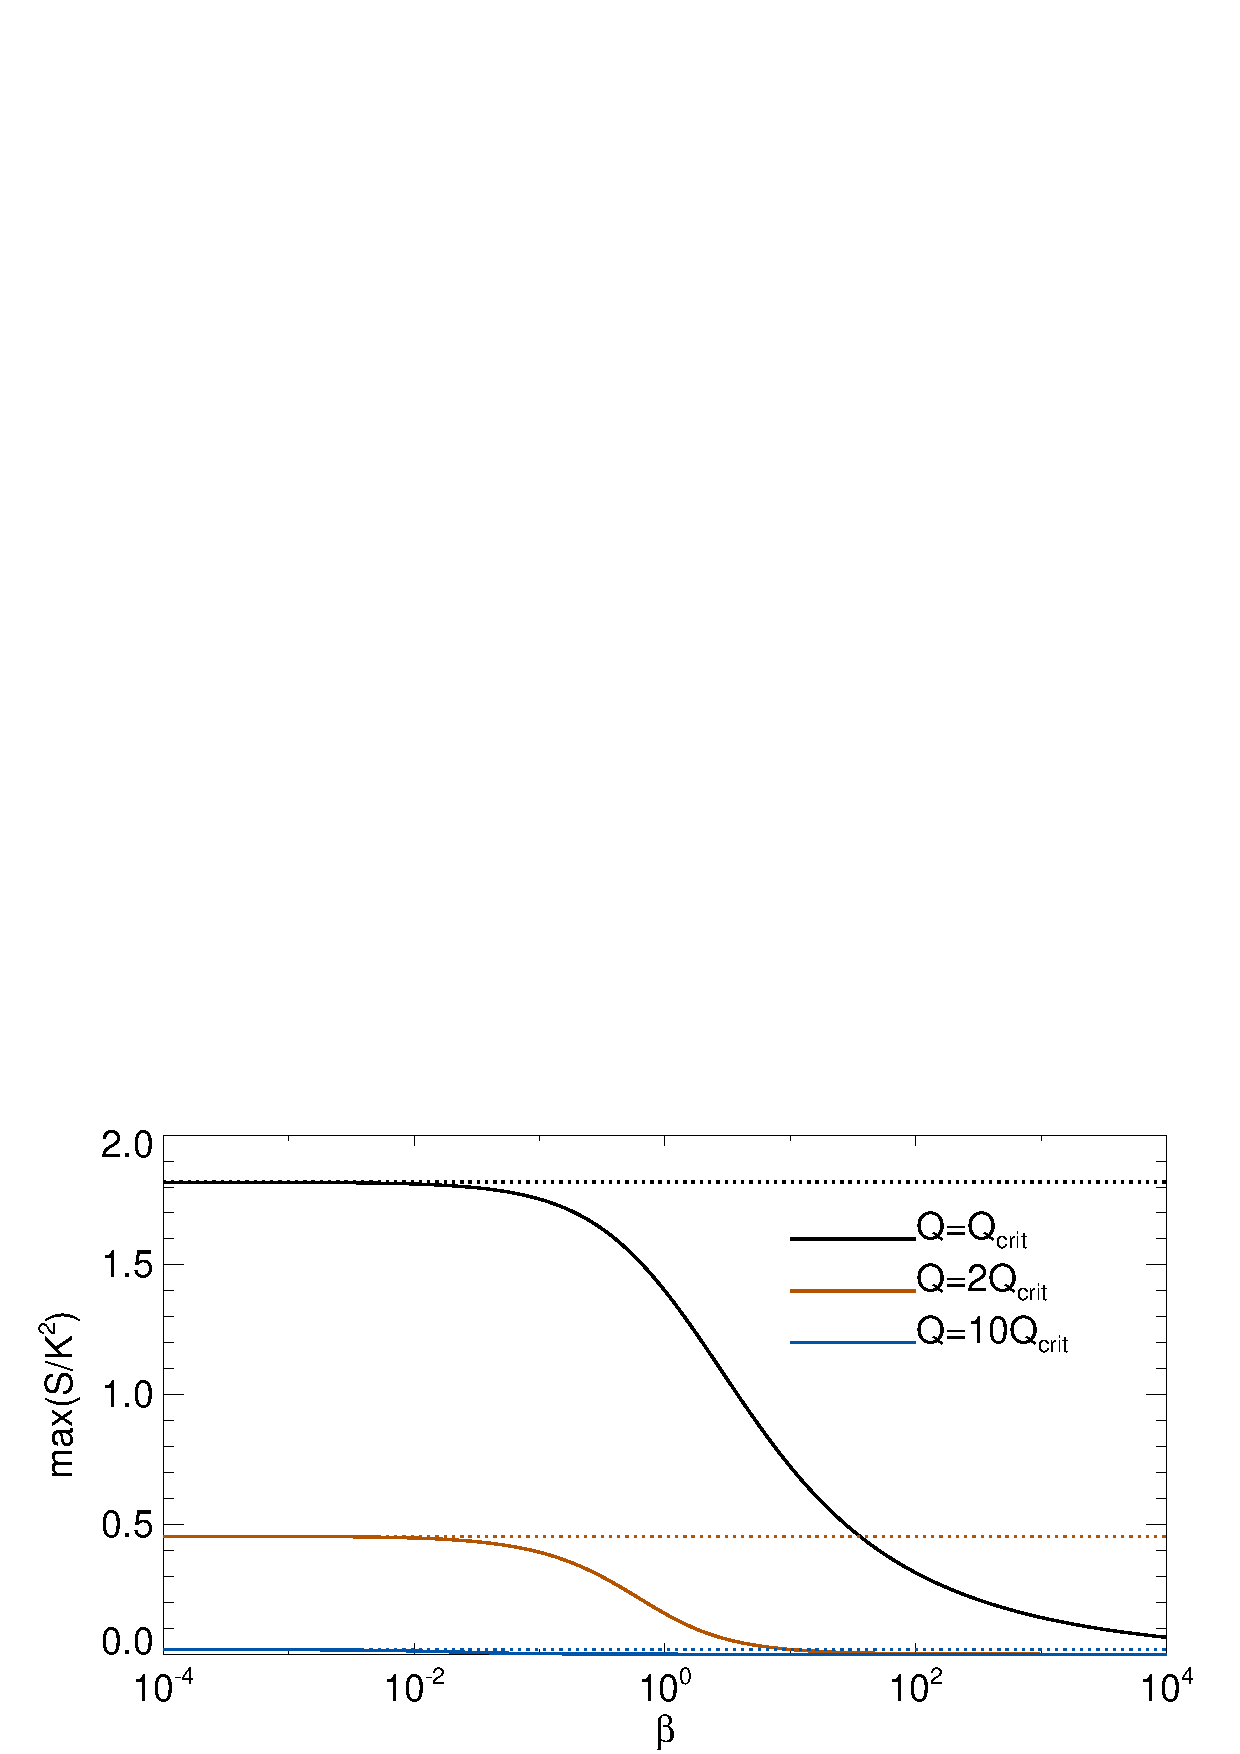
\includegraphics[width=\linewidth,clip=true,trim=0cm 0cm 0cm 0.8cm]{figures/inviscsg_alpha}
%  \caption{A measure of the
%    associated stress that can be expected in the non-linear
%    regime. The horizontal dotted lines
%    correspond to Eq. \ref{max_alpha}.}
%\end{figure}

\subsection{Viscous disk}\label{2dvisc}
We now consider a viscous disk with 
$\mu=-1,\,\lambda=0$ as discussed in \S\ref{visc_model}. We first
check in Appendix \ref{gammie_check} that our dispersion relation
reduces previous results in the adiabatic/isothermal limit.  

To see the effect of finite cooling, we simplify the dispersion relation,
Eq. \ref{thindisk}, by assuming $|\beta S|\ll 1$. Then  
for $|K| \to 0$ we find
\begin{align}\label{gammie_smallk}
%  S \sim \frac{\alpha |K|^3}{(2-q)Q},%derived assuming |beta*S|<<1 
%  S \sim \frac{\alpha K^2\left[2|K|Q^{-1} - \gamma K^2 + 2\alpha q
%    (2-q)(\gamma-1)K^2\right]}{2(2-q)+\gamma K^2 - 2|K|Q^{-1}} %derived
                                %assuming |\beta S|>>1
  S\simeq \frac{\alpha K^2}{2(2-q)}\left(\frac{2|K|}{Q} - \theta
  K^2\right), 
\end{align}
which coincides with \citeauthor{gammie96}'s Eq. 18 for vanishing
wavenumber. For $|K|\to\infty$ we find
\begin{align}\label{gammie_bigk}
  %  S \sim \frac{2}{Q|K|}\left(\frac{4}{3}\alpha + \gamma\beta\right)^{-1}.
  S \simeq\left(\frac{2}{Q|K|} - \theta\right)\left(\frac{4}{3}\alpha + 
  \alpha_b + \gamma\beta\right)^{-1}.
\end{align}



For $\theta\ll1$ a rough measure of the maximum growth rate can be obtained by
equating Eq. \ref{gammie_smallk} and \ref{gammie_bigk}\footnote{If
  $\theta$ is not small and/or $Q$  is large then one may just use Eq. \ref{gammie_smallk}
  to maximize $S$ over $K$, see the $\theta=0.3,\beta=100$ curve in the bottom
  panel of Fig. \ref{gammie_rate_plot}}.  
This exercise yields 
\begin{align}\label{gammie_maxrate_simple}
  %S_* \simeq
  %\frac{1}{Q}\left(\frac{\alpha}{2-q}\right)^{1/4}\left(\frac{6}{4\alpha
%+ 3\gamma\beta}\right)^{3/4}. 
  S_*\simeq \frac{
    6^{3/4}\left[\alpha\left(4\alpha +
      3\alpha_b + 3\gamma\beta\right)\right]^{1/4} - 3\theta
    Q(2-q)^{1/4}}{Q\left(4\alpha + 3\alpha_b +
    3\gamma\beta\right)(2-q)^{1/4}}. 
\end{align} 
%gravito-viscous instability 

As a numerical example, we consider a model with $\alpha_b=0$ and
$\alpha=\alpha(\beta)$ given by thermal equilibrium (
Eq. \ref{alpha_beta_relation}). Furthermore, we relate 
\begin{align}
  Q = \frac{Q_\mathrm{crit}}{\sqrt{\alpha}},\label{Qalpha}
\end{align}
to mimic a basic state maintained by gravito-turbulence where one
might expect the dimensionless stress $\alpha \sim Q^{-2}$
\citep{lin87}.   

Fig. \ref{gammie_rate_plot} show growth rates as a function of the
wavenumber $k$ obtained from the dispersion relation
Eq. \ref{thindisk}. The limiting behavior for small/large $K$ are
well-captured by Eq. \ref{gammie_smallk} and
\ref{gammie_bigk}. Comparing the two panels shows that increasing the
irradiation level ($\theta$) surpresses small-scale perturbations.     

\begin{figure}
  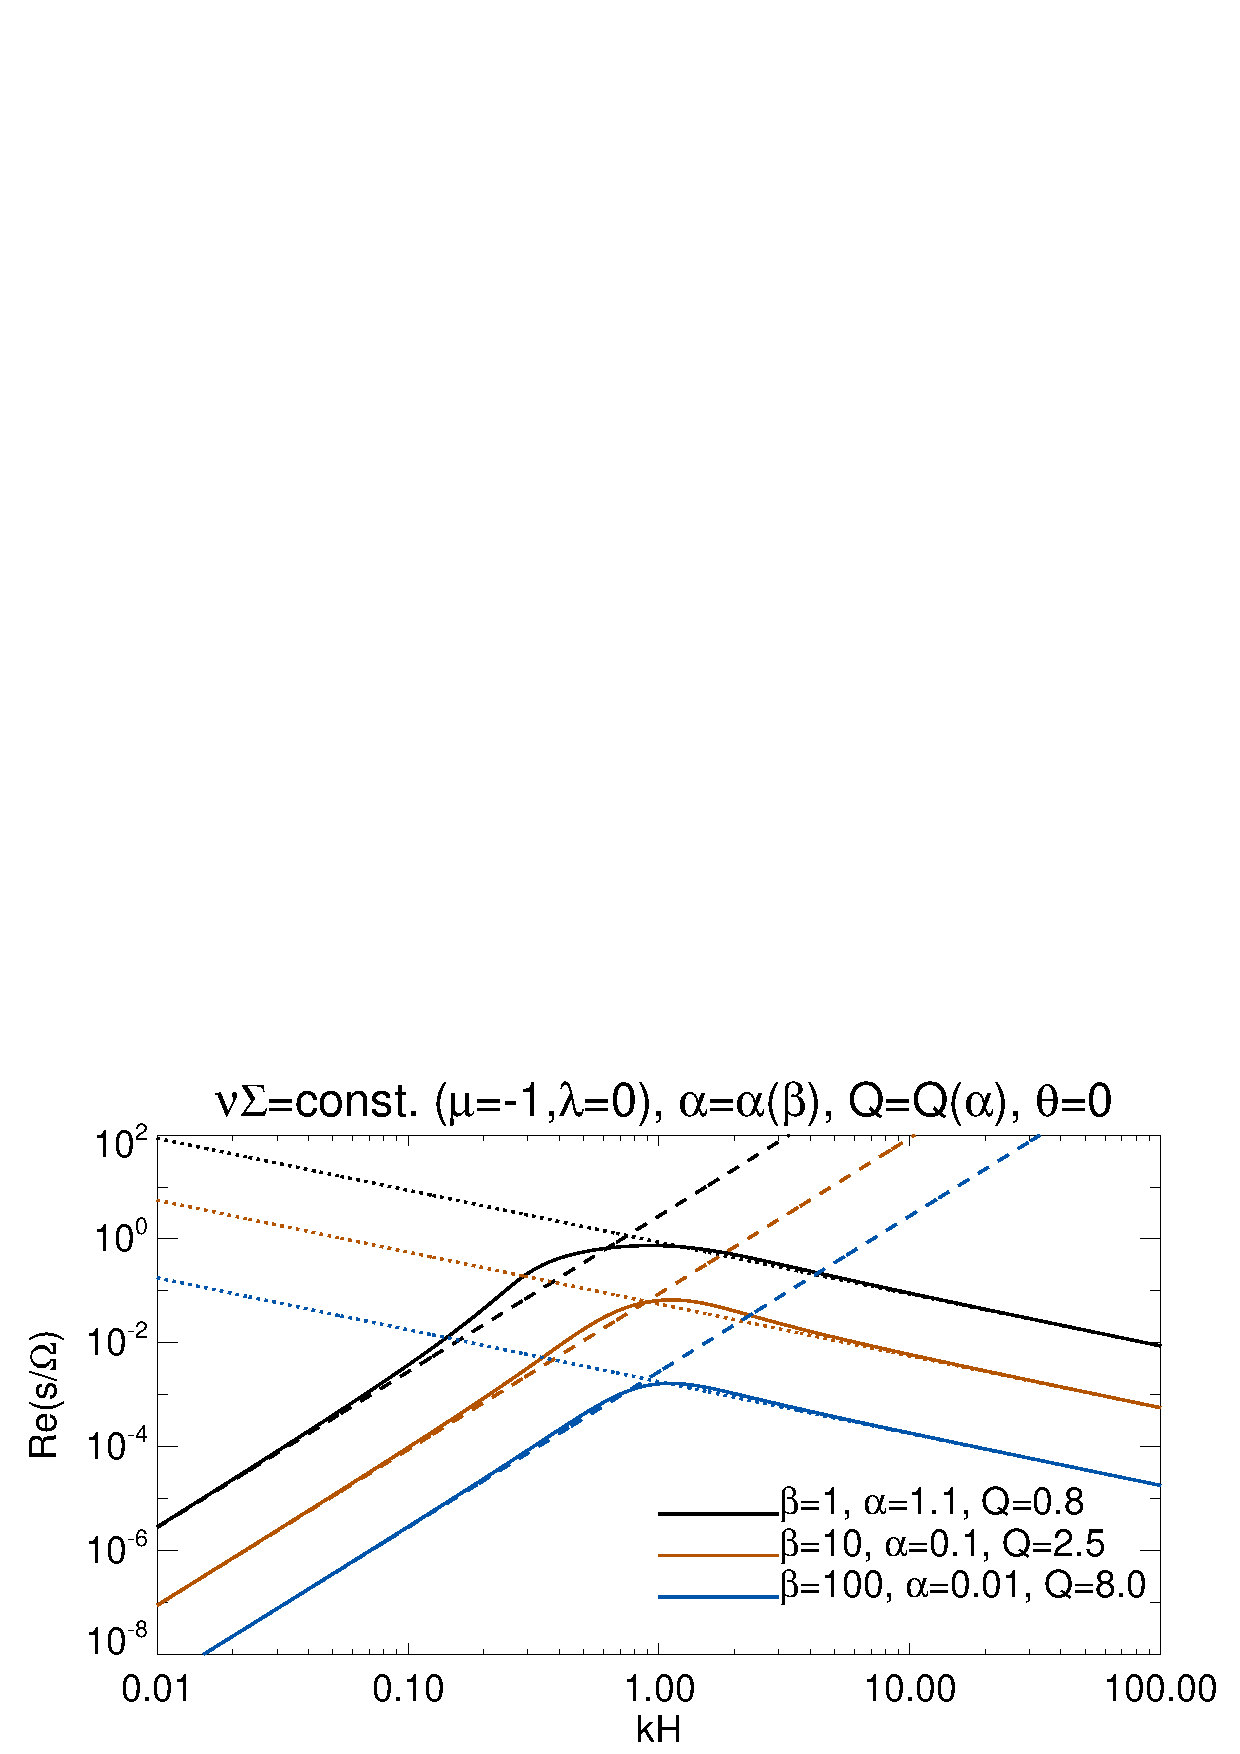
\includegraphics[width=\linewidth,clip=true,trim=0cm 1.5cm 0.4cm
    0.0cm]{figures/viscsg_modes}\\
  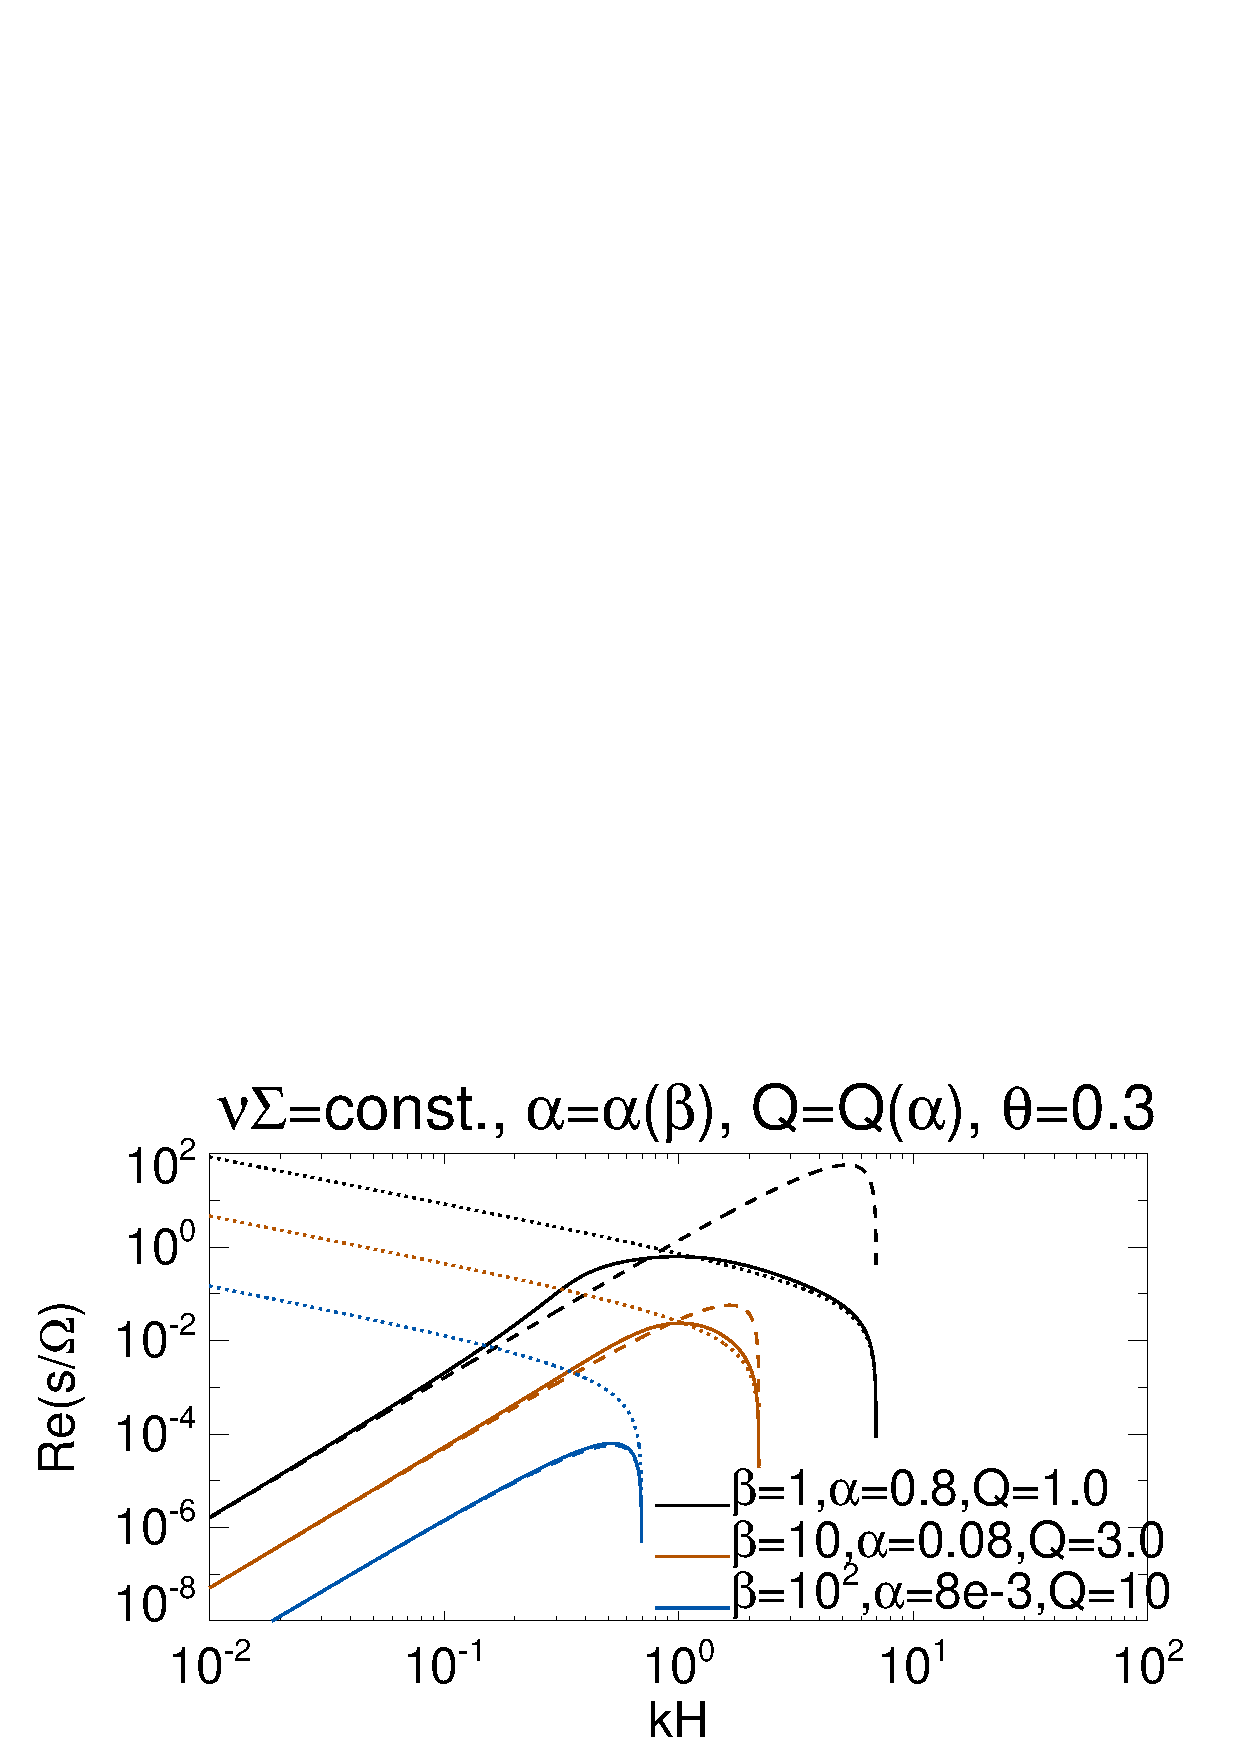
\includegraphics[width=\linewidth,clip=true,trim=0cm 0cm 0.4cm
    0.0cm]{figures/viscsg_modes_theta0d3}
  \caption{Growth rates for the 2D viscous problem as a function of
    the radial wavenumber $k$ for a range of cooling times
    $\beta$. The dashed and dotted lines correspond to asympototic
    behaviors for small and large $k$, respectively, computed from
    Eq. \ref{gammie_smallk} and \ref{gammie_bigk}. Top: without
    irradiation, bottom: partially irradiated disk. 
    \label{gammie_rate_plot}}
\end{figure}


Fig. \ref{gammie_maxrate_plot} shows the maximum
growth rate (top panel) and the corresponding wavenumber (bottom
panel) as a function of the cooling time $\beta$ for $\theta=0$.  
There is good agreement between numerical growth rates and
Eq. \ref{gammie_maxrate_simple} for $\beta \gtrsim 1$. 
%The assumption
%of $|\beta S|\ll 1$ is not well satisfied at smaller $\beta$ which
%explains the mismatch there. 
Eq. \ref{gammie_maxrate_simple} gives the
limiting behavior for this case as   
\begin{align*}
  S_*\propto \begin{cases}
%    \frac{\alpha^{1/4}}{Q\beta^{3/4}} \propto \beta^{-3/2} 
    \alpha^{1/4}\beta^{-3/4}Q^{-1}\propto \beta^{-3/2} 
    &  \beta \gg \alpha, \\
%    \frac{1}{Q\sqrt{\alpha}}  
    \alpha^{-1/2}Q^{-1} = \mathrm{const.} & \beta \ll \alpha,    
  \end{cases}
\end{align*}
where we have applied Eq. \ref{alpha_beta_relation}
and \ref{Qalpha}. The disk is formally unstable for all $\beta$, but
growth timescales are long ($>10$ orbits) for $\beta \gtrsim
20$. This region is marked by the vertical dashed-dotted line in
Fig. \ref{gammie_maxrate_plot}. The optimum wavenumber decreases with
the cooling time for $\beta\lesssim O(1)$ because larger scales are
more resistant to the associated increase in viscous damping.      

{\bf maybe move following to discussion}
Numerical simulations of self-gravitating disks show there is a
maximum $\alpha$ ($\sim 0.06$) that can be sustained before
fragmentation \citep{rice11}. We can interpret this result in our
linear framework. 
%We can use our case (\ref{gvisc}) to interpret this
Suppose it is possible to balance rapid cooling ($\beta\lesssim1$) 
by generating a large gravito-turbulent heating rate
($\alpha\gtrsim 1$) through a small $Q$. Fig. \ref{gammie_maxrate_plot} 
shows that such a system would be dynamically unstable with 
growth rate $s = O(\Omega)$. This due to the direct effect of viscous 
stress promoting instability, rather than cooling. Thus, we do not expect rapidly-cooled, 
and hence highly turbulent, self-gravitating disks to persist beyond
dynamical timescales. This is consistent with previous numerical
simulations performed by \cite{lodato05}. 
%Case (\ref{gvisc}) is consistent with 
\begin{figure}
%  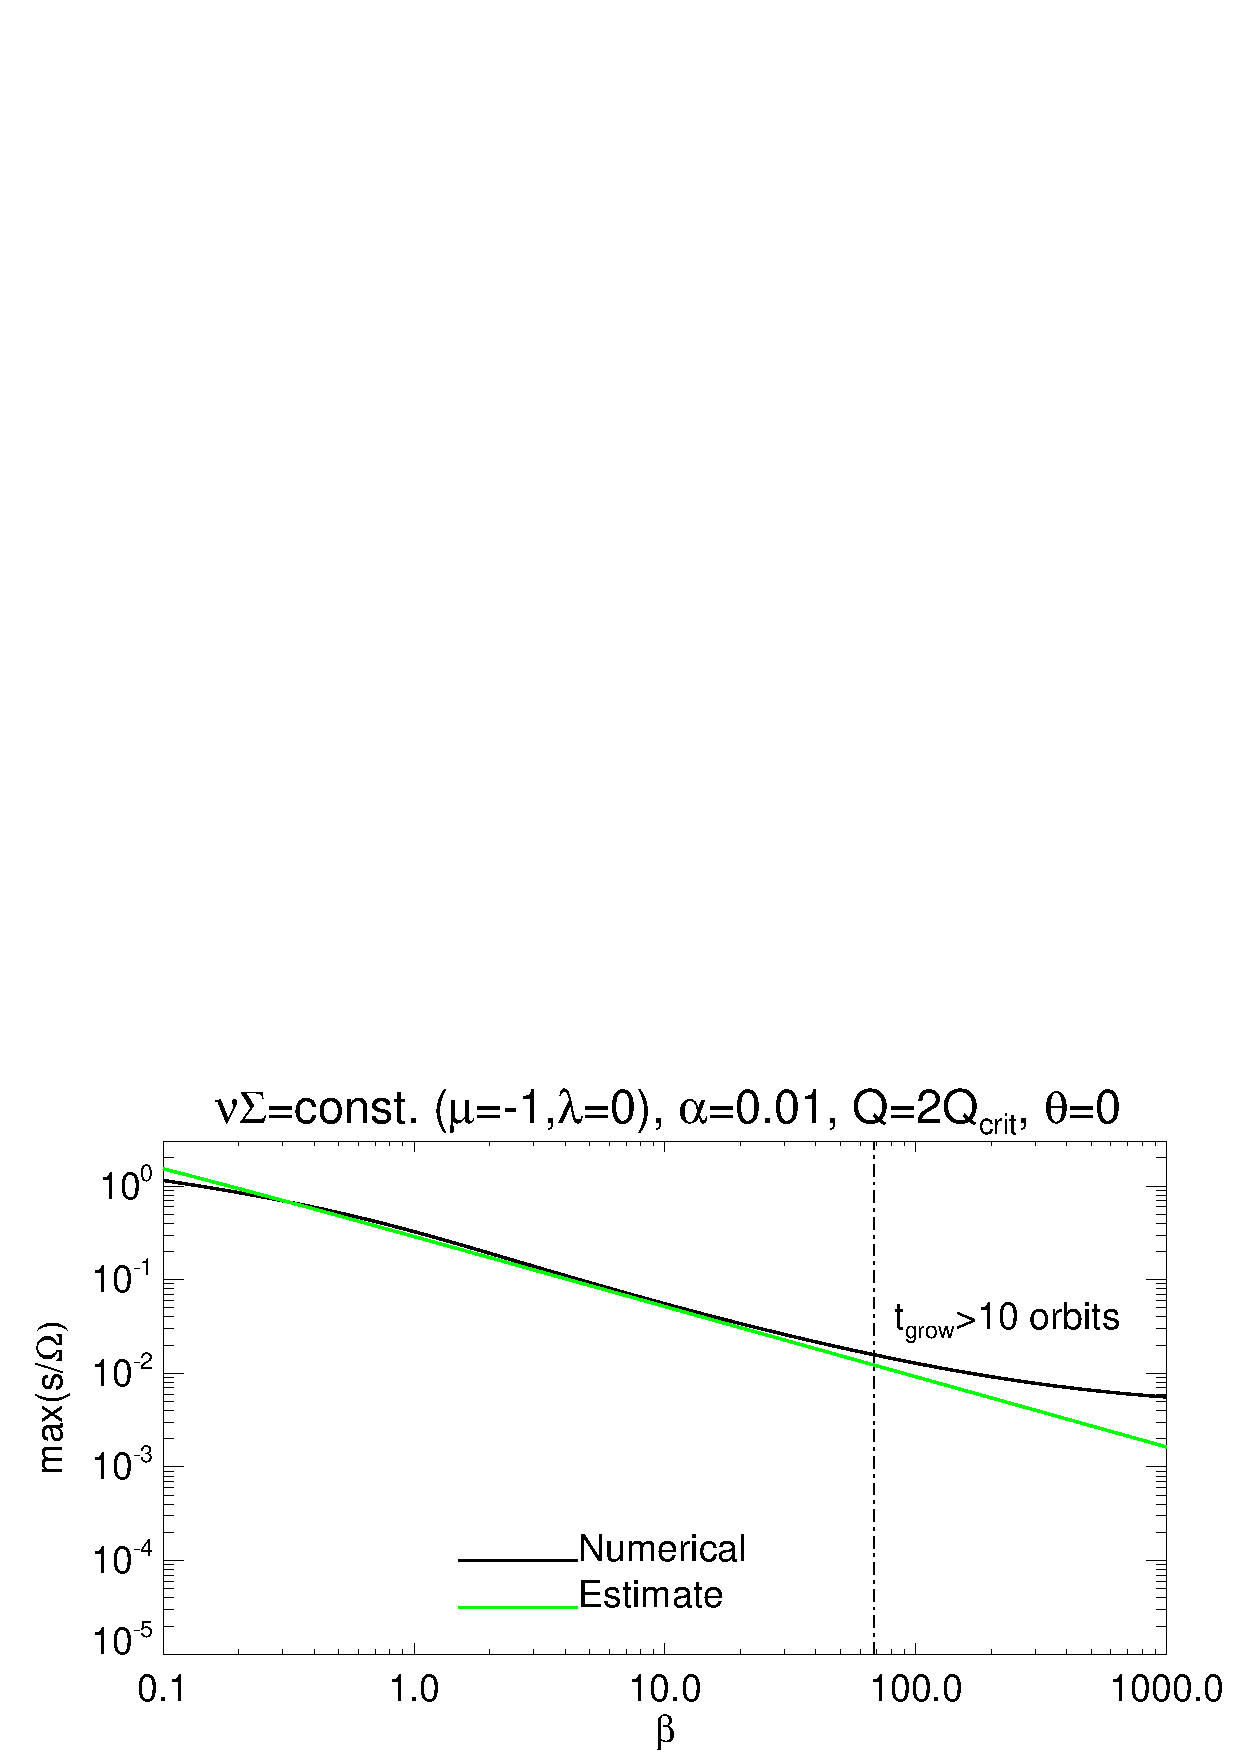
\includegraphics[width=\linewidth,clip=true,trim=0cm 1.5cm 0cm
%    0.0cm]{figures/result2d_fixalpha}\\
%  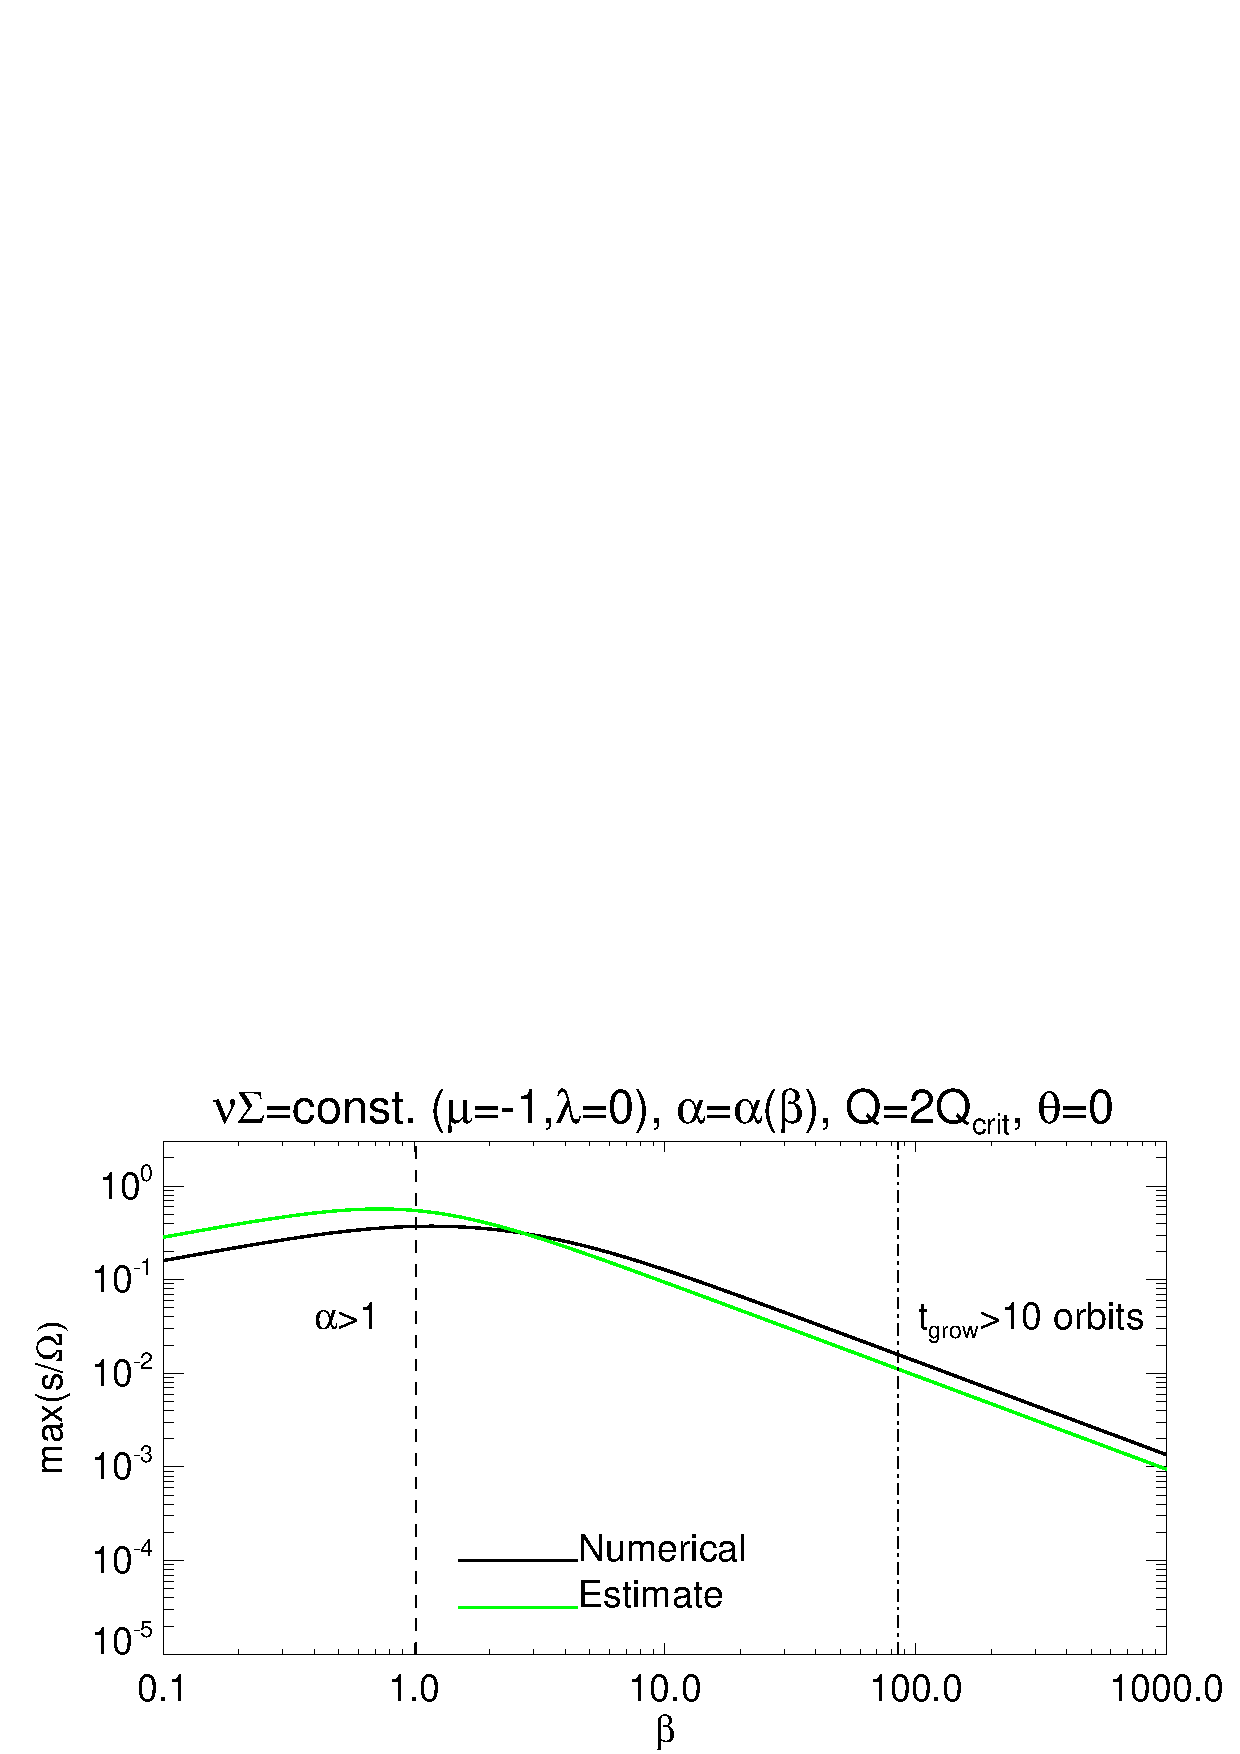
\includegraphics[width=\linewidth,clip=true,trim=0cm 1.5cm 0cm
%    0.0cm]{figures/result2d_fixQ}\\
  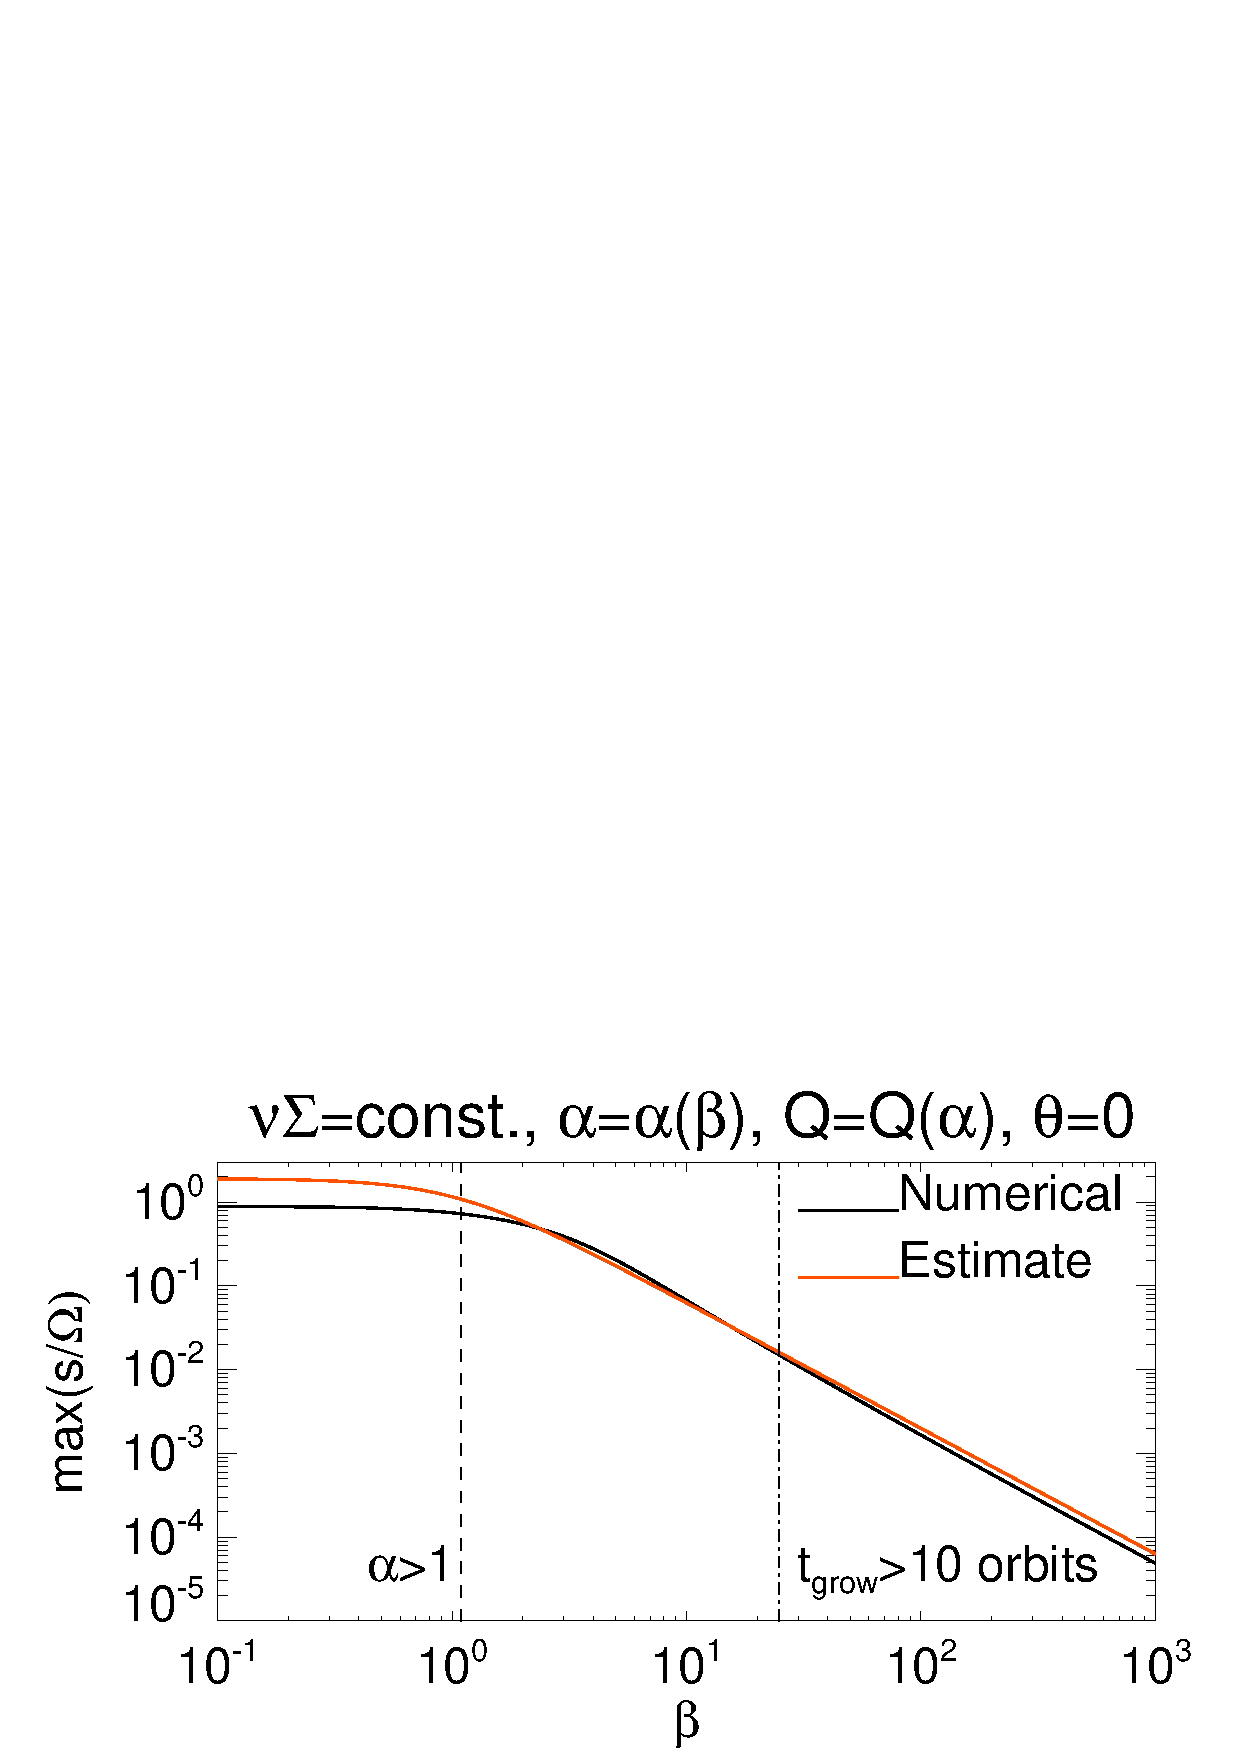
\includegraphics[width=\linewidth,clip=true,trim=0cm 1.5cm 0.cm
    0.0cm]{figures/result2d_gvisc}
  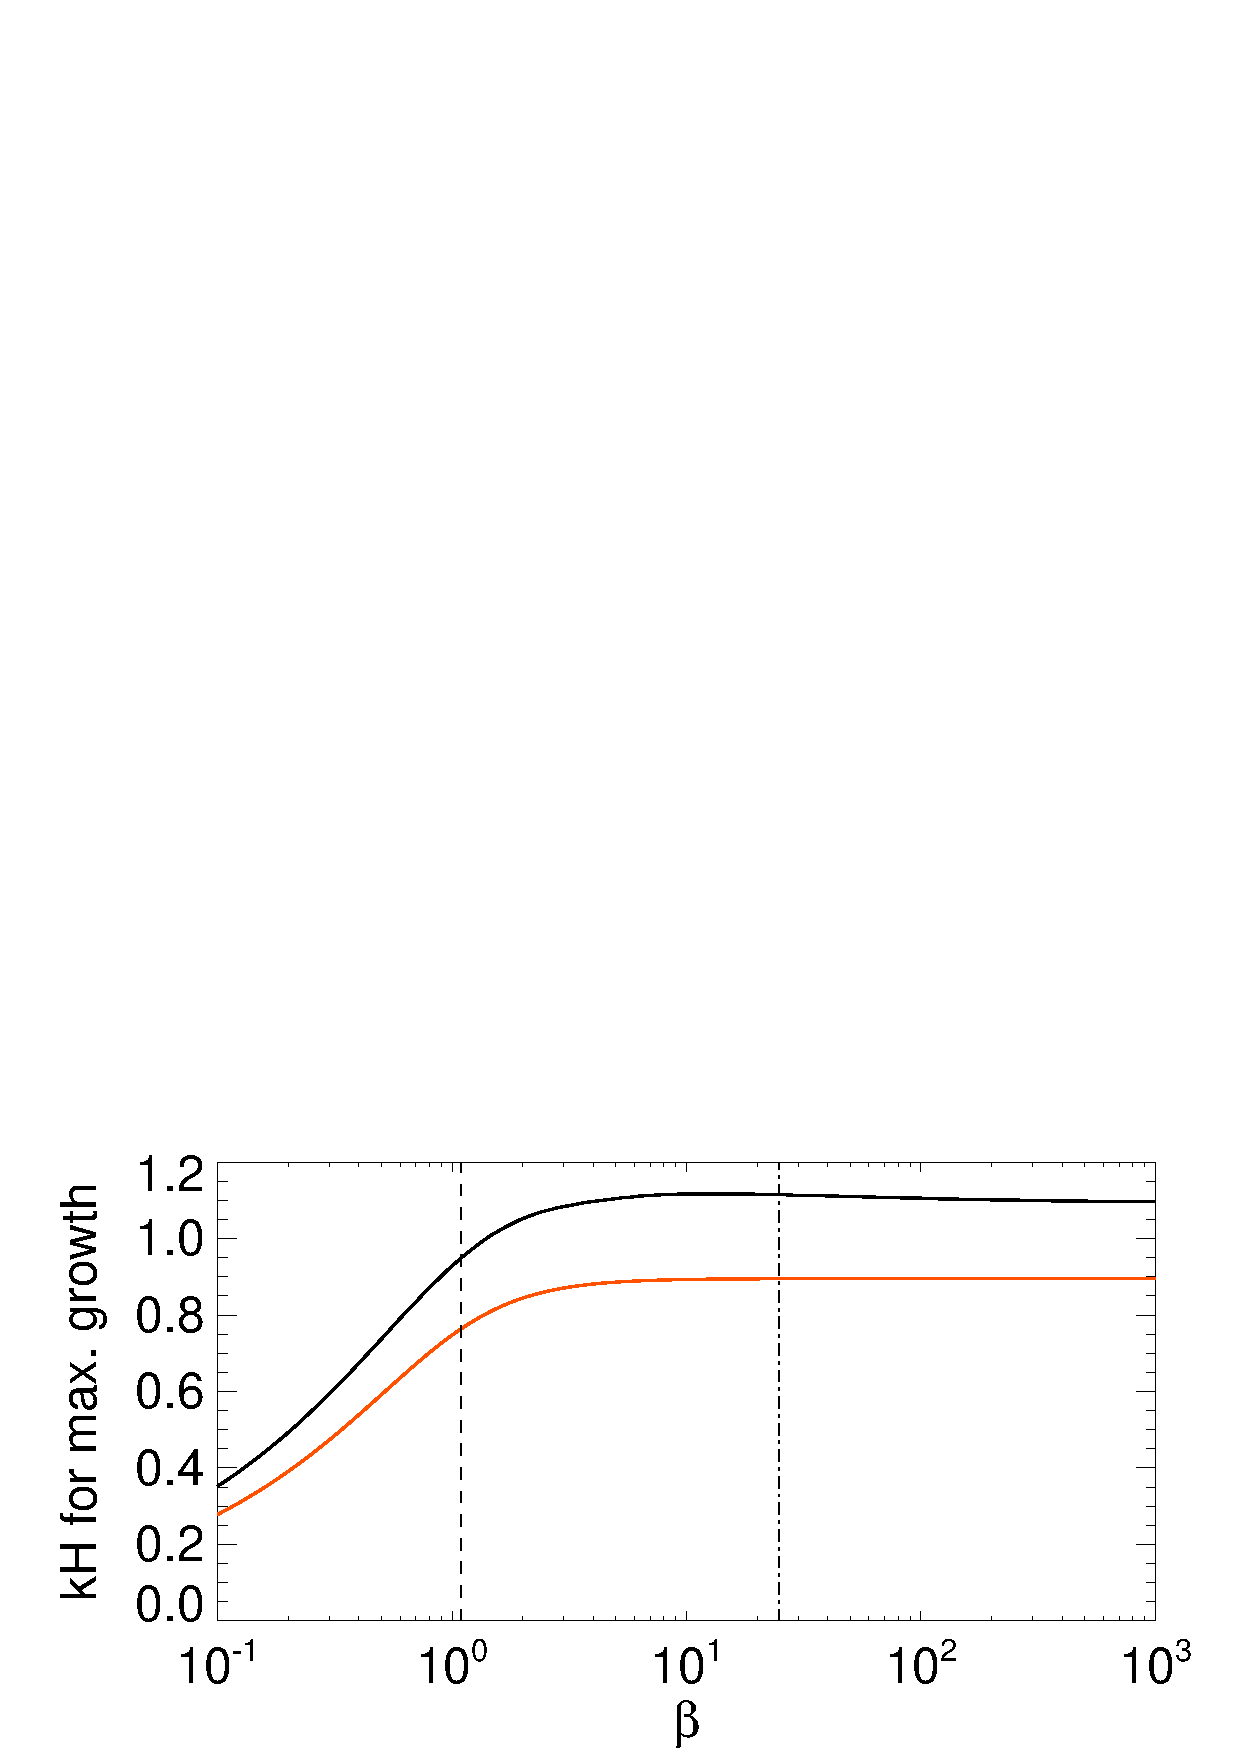
\includegraphics[width=\linewidth,clip=true,trim=0cm 0cm 0.cm
    1.0cm]{figures/result2d_gvisc_kmax}
  \caption{Growth rates (top) at the optimal wavenumber (bottom) for
    viscous GI as a function of cooling time for the
    case shown in Fig. \ref{gammie_rate_plot}. Solid lines are
    computed from the dispersion relation (Eq. \ref{thindisk}), and the dotted line is an
    estimate from Eq. \ref{gammie_maxrate_simple}. The vertical dashed
    line marks the region with $\alpha > 1$, and the vertical
    dashed-dot line marks the region with growth timescales longer
    than dynamical. 
    \label{gammie_maxrate_plot}}
\end{figure}

\section{Three-dimensional disks with beta cooling}\label{3ddisk}
We confirm the above results in 3D disks with vertical
structure. Accounting for the third dimension will weaken gravitational instabilities
because the disk mass is spread across some vertical extent. It is 
possible to incorporate this effect in the previous 2D framework, but doing so
introduces an additional `softening' parameter $H_\mathrm{sg}$ as discussed in
Appendix \ref{3dcorr}. It is more direct to solve the 3D eigenvalue
problem to avoid such uncertainties. Our numerical approach is
outlined in Appendix \ref{3d_method}. 

%We will find that while softening the
%self-gravity in 2D can produce qualitatively similar results to 3D, a
%quantitative match is  
%{\bf note: fast beta-cooling in 3D destablizes vertical modes (enables
%convection)}
%take k>0 wlog
%consider Gamma=1
%height s.t. rho(zmax) = 0.05 rho(0) avoid very low densities 

In the following examples we consider a vertically isothermal disk
($\Gamma=1$ in Eq. \ref{poly_vert}). Then in the viscous case $\alpha$ is vertically
constant (Eq. \ref{alpha_beta_relation}). We consider only even modes
about the mid-plane, and apply a numerical disk surface at $z=\zmax$
such that $\rho(\zmax)=0.05\rho_0$.     

%in practice eliminate density with poisson
\subsection{Inviscid 3D disk}

We consider a 3D inviscid disk with $\gamma=1.4$, $\qthree=0.71$, and $\theta=0$. 
The 3D gravity parameter $\qthree$ is defined by 
Eq. \ref{Q3d_def}. For such a disk, the corresponding Toomre parameter 
$Q=2Q_\mathrm{crit}$. Recall $Q_\mathrm{crit}$, defined by
Eq. \ref{qcrit_def}, is the Toomre parameter value such that the 2D
disk would be marginally stable in the absence of cooling. 

Fig. \ref{3d_inviscid} shows growth rates and the most unstable
wavenumbers obtained for this model. We also plot 2D
results with the 3D correction as described in Appendix
\ref{3dcorr}. The (empirically) chosen value of 
$H_\mathrm{sg}=0.64H$ results in a close match between 2D and 3D
growth rates, but the most unstable wavenumber in 3D is somewhat smaller. 
This offset reflects self-gravity being weakened in the vertical 
direction: a larger horizontal scale is required to achieve the same
strength of self-gravity as the 2D case. Similarly, 
choosing $H_\mathrm{sg}=0.53H$ matches the optimum wavenumbers, but
growth rates are over-estimated in 2D.    

\begin{figure}
  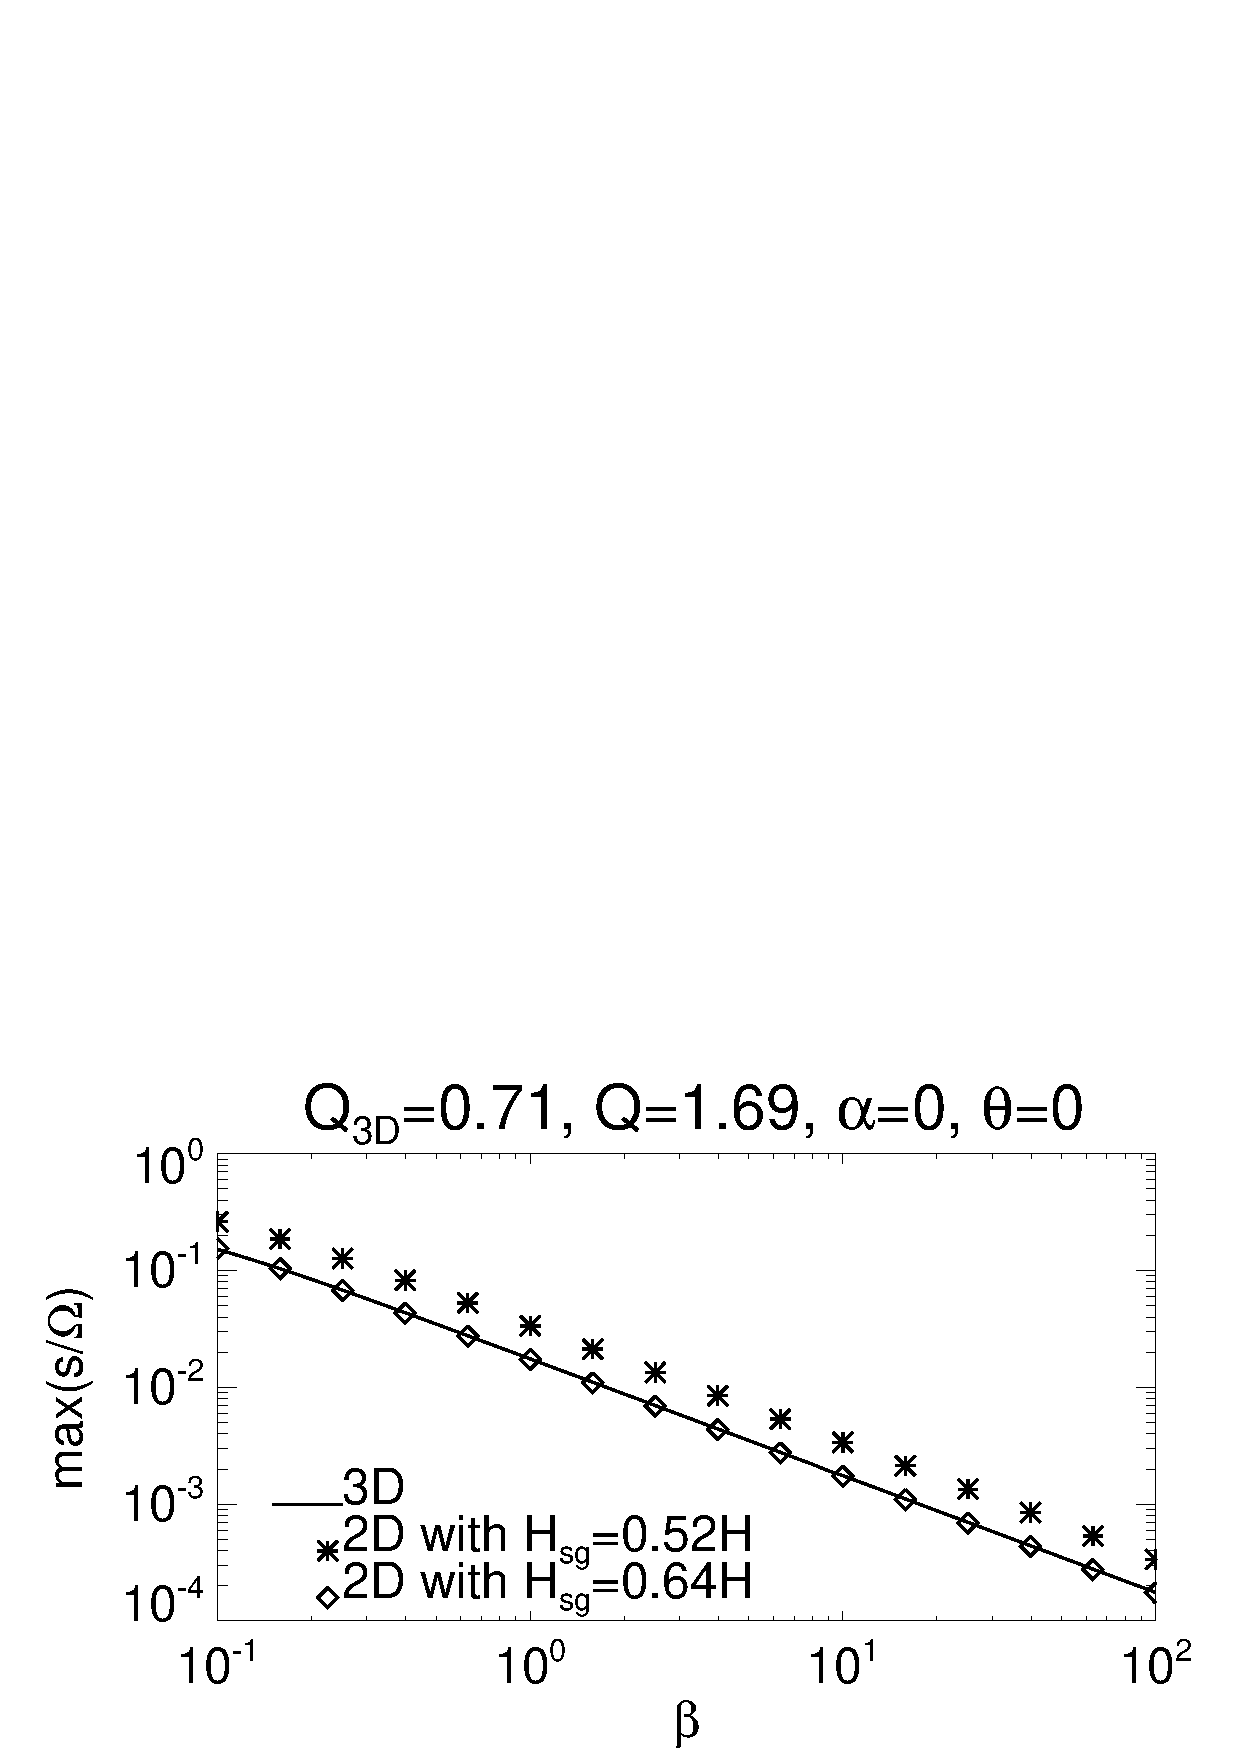
\includegraphics[width=\linewidth,clip=true,trim=0cm 2cm 0.cm
    0.0cm]{figures/3d_inviscid_rates}\\
  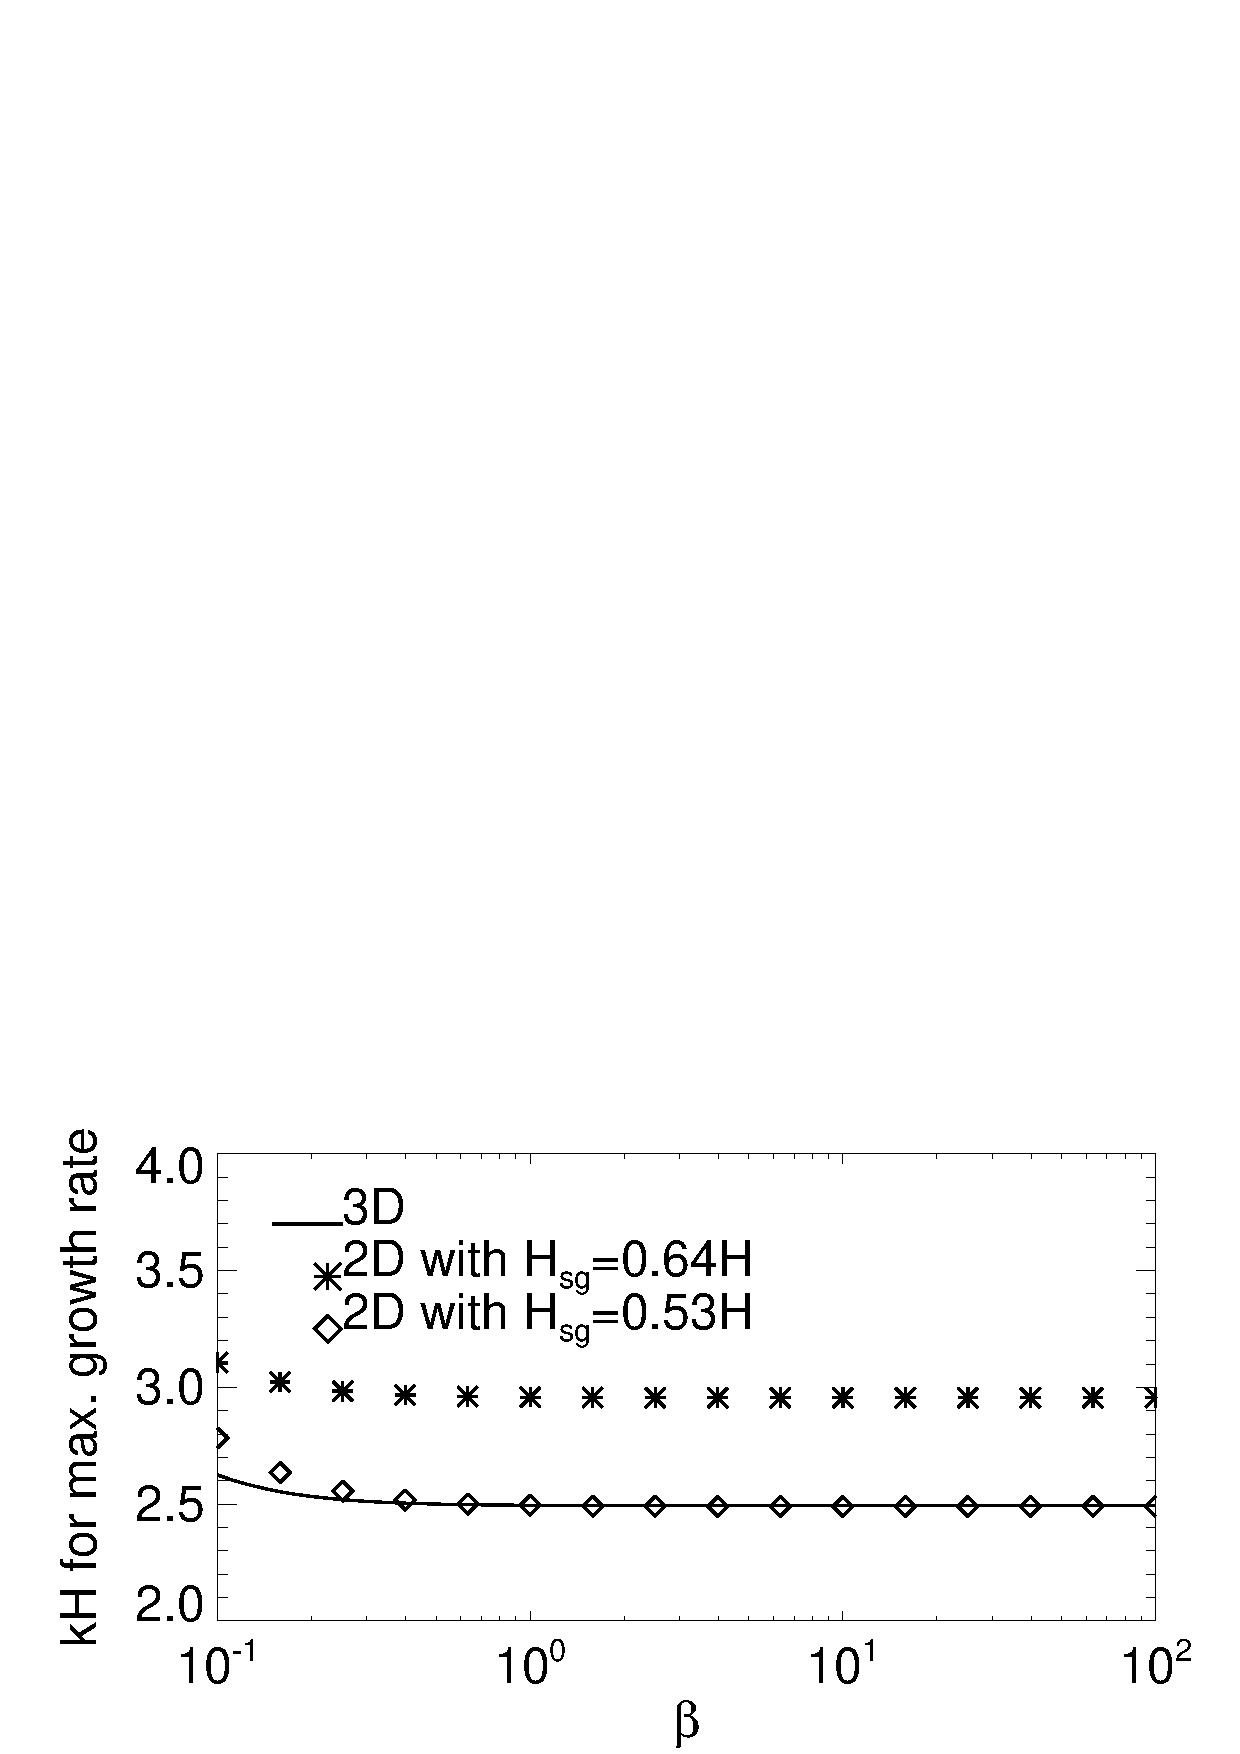
\includegraphics[width=\linewidth,clip=true,trim=0cm 0cm 0.cm
    0.8cm]{figures/3d_inviscid_kmax}
  \caption{Growth rates (top) and optimal wavenumber (bottom) obtained
    from the inviscid 3D eigenvalue problem (solid line). Asterisks
    and diamonds are corresponding values from the 2D dispersion
    relation (Eq. \ref{thindisk}) but with a softened gravity as
    described in Appendix \ref{3dcorr}. \label{3d_inviscid}} 
\end{figure}

\subsection{Viscous 3D disk} %growth rates, kmax, eigenfunction
For the 3D viscous problem we use the same set up as that in 2D
(\S\ref{2dvisc}), but with 
\begin{align}
  \qvert = \frac{Q_\mathrm{3D,crit}}{\sqrt{\alpha}}, \label{Q3d_visc_model}
\end{align}
where $Q_\mathrm{3D,crit}\simeq0.36$ is the 3D equivalent to the 2D
critical value, $Q_\mathrm{crit}$. Note that the background vertical
structure now varies with $\alpha$ through Eq. \ref{Q3d_visc_model},
which in turn depends on the cooling time through thermal
equilibrium (Eq. \ref{alpha_beta_relation}). 

Fig. \ref{3d_visc} shows growth rates, maximized over $k$, as a
function of the cooling time $\beta$. We also plot 2D results with 3D
corrections. Softening the self-gravity in 2D captures the correct 
qualitative behavior of the full 3D case. For $\beta\gtrsim 1$
choosing $H_\mathrm{sg}=0.8H$ produces a good match. However, it is
clear that a single, constant value of $H_\mathrm{sg}$ cannot
re-produce 3D growth rates for all $\beta$. This suggests that the
exact value of $H_\mathrm{sg}$ is problem-dependent, although taking 
$H_\mathrm{sg}\sim O(H)$ should give the correct 3D growth rate within 
a factor of two. 
%cooling helps vertical modes (convection) 
%slower variation wrt z for low beta because of associated high
%viscosity
%smooth out vertical gradients 


Fig. \ref{3d_visc_vz} shows the magnitude of the vertical velocity 
$|\delta v_z|$ scaled by the total horizontal velocity for $\beta =
1,\,10$ and $100$. Vertical speeds are sub-dominant at $\lesssim 30\%$
of the total horizontal speeds. 
{\bf These vertical velocities are associated with viscous
  GI, and should not be compared with that associated with the
  underlying gravito-turbulence \citep[e.g.][]{shi14},
  which is neglected in our framework when defining the basic state.   
}
%This suggests that it is not essential 
%to consider 3D models when considering gravitational instabilities. 
%{\bf KMK this is not true generically, so
%this statement needs to be more specific or cut}.

\begin{figure}
  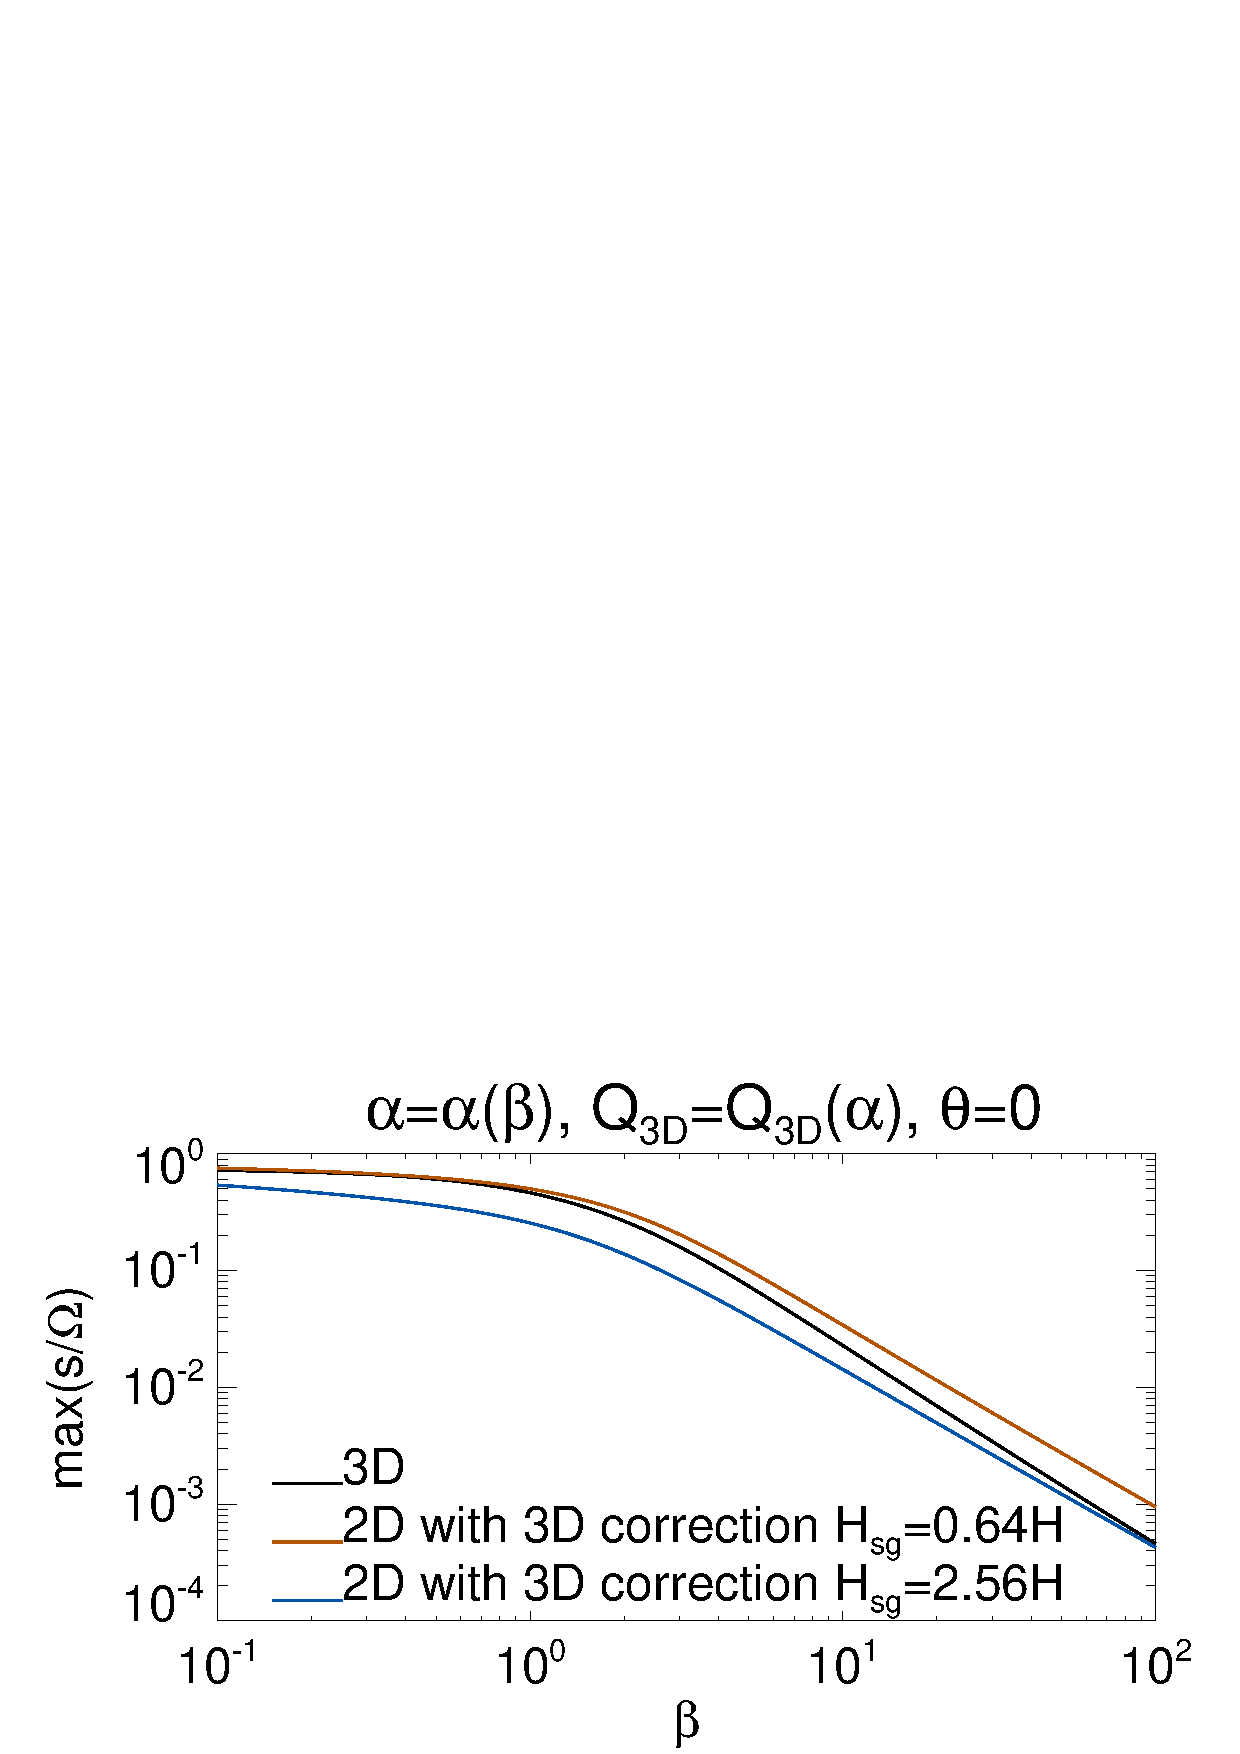
\includegraphics[width=\linewidth,clip=true,trim=0cm 0.cm 0.cm
    0.0cm]{figures/growth_visc3d}
  \caption{Growth rates from the viscous 3D eigenvalue problem (black solid
    line). Asterisks and diamonds are obtained from the 2D dispersion
    relation (Eq. \ref{thindisk}) with softened gravity as described
    in Appendix \ref{3dcorr}. \label{3d_visc}} 
\end{figure}



\begin{figure}
  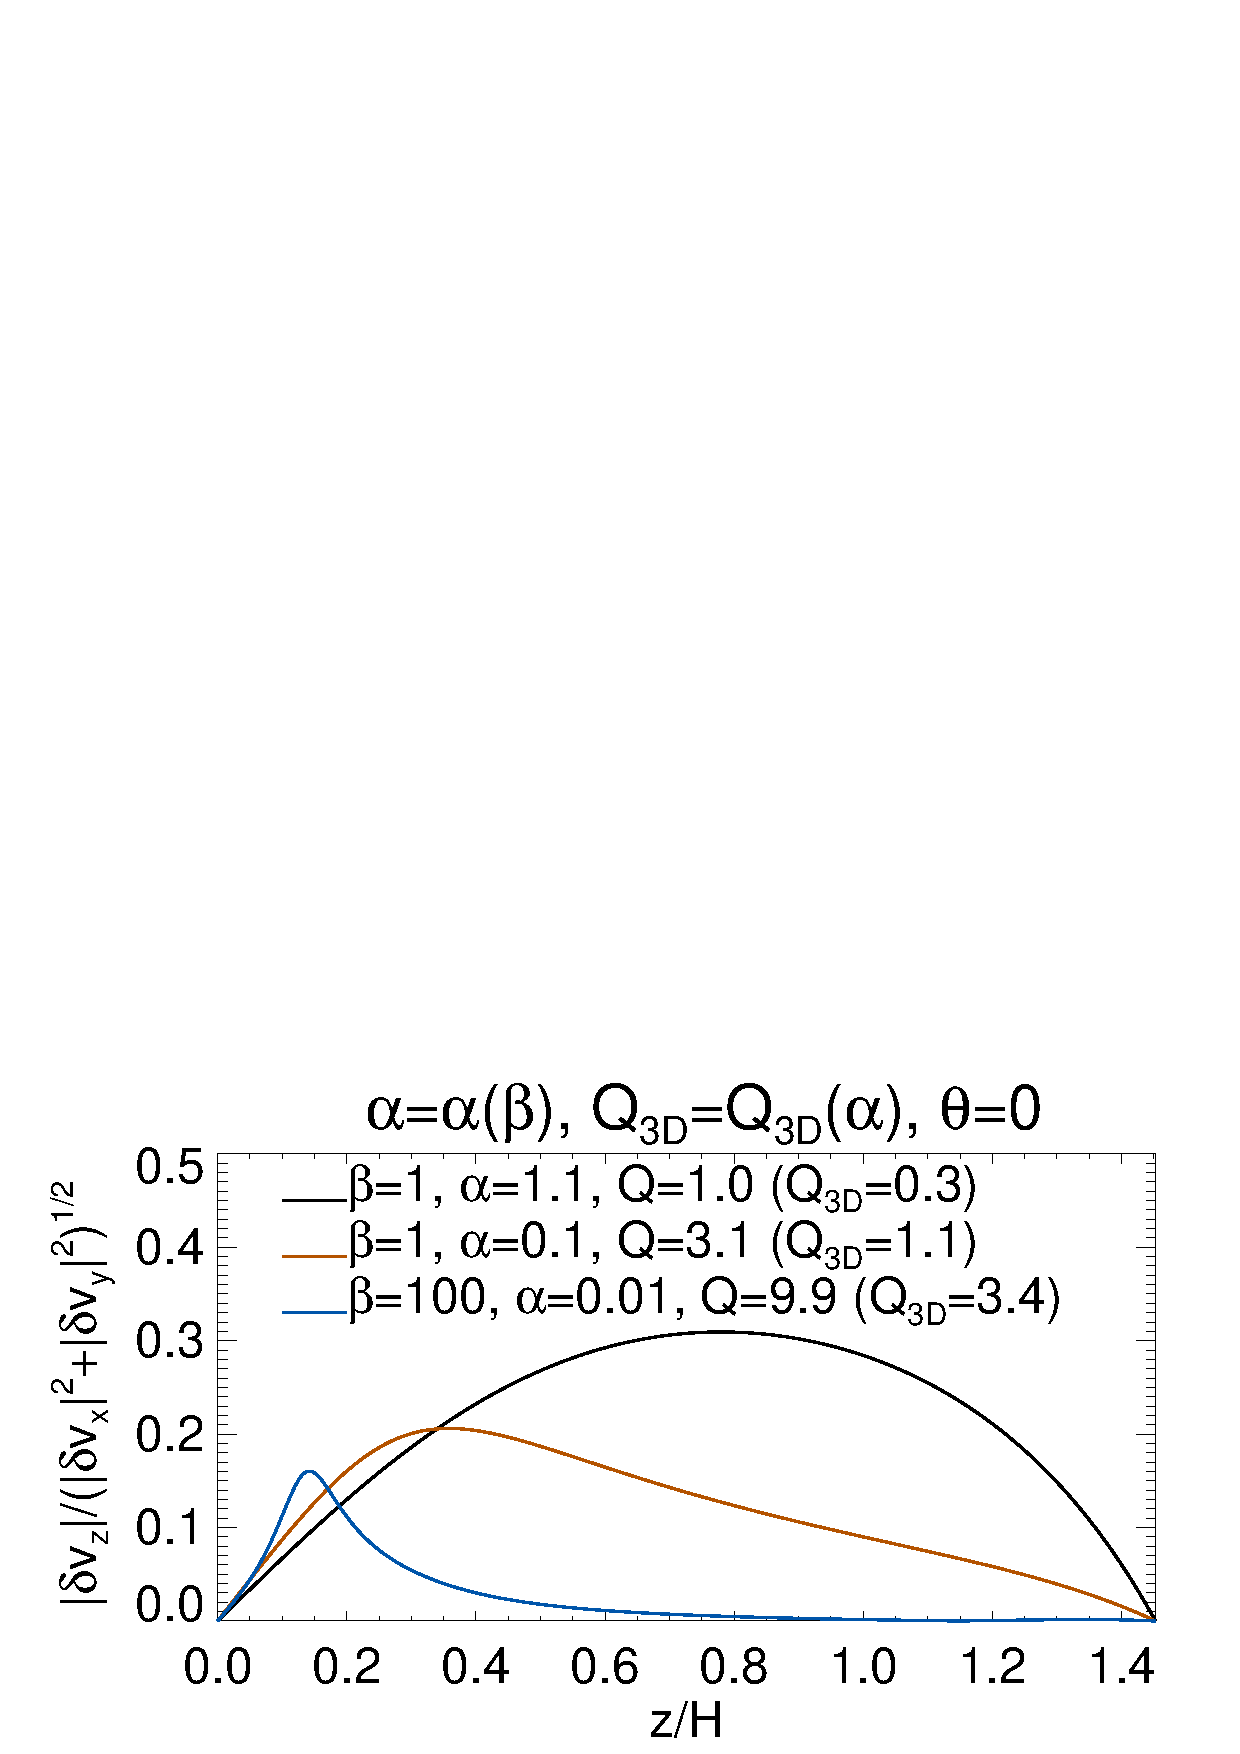
\includegraphics[width=\linewidth,clip=true,trim=0cm 0.cm 0.cm
    0.0cm]{figures/eigenvec_vz}
  \caption{Magnitude of vertical velocities, normalized by the
    magnitude of the total horizontal velocity, of the viscous GI in 
    Fig. \ref{3d_visc}, for three cooling times: $\beta=1,\,10$, and $100$. \label{3d_visc_vz}} 
\end{figure}

\section{Application to protoplanetary disks}\label{2dppd}
We now apply our linear framework to assess the stability of  
protoplanetary disks. We consider the gravito-turbulent disk models recently
developed by \cite[][hereafter \citetalias{rafikov15}]{rafikov15}. 
This 2D, Keplerian disk orbits a Solar 
mass star and is defined by the following parameters, 

\begin{itemize}
  \item $\dot{M}$, the global radial mass accretion rate;
  \item $Q_0$, the value of the 2D Toomre parameter where the disk is
    gravito-turbulent;
  \item $T_\mathrm{irr}$, the irradiation or floor temperature;
  \item $\alpha_m$, the dimensionless viscosity associated with other
    sources of turbulence, such as magneto-rotational instabilities
    (MRI, see also \S\ref{visc_gi} and \S\ref{MHD}). 
\end{itemize} 
These are used in the statements of thermal equilibrium, mass and
angular momentum conservation, together with an opacity law, 
to construct a global disk model with surface density $\Sigma(R)$ and
temperature $T(R)$ where $R$ is the global cylindrical radius from the
star. \citepalias[See][for details.]{rafikov15} This gives the $Q(R)$
value required for input into our linear framework. We derive other
dimensionless parameters below. 

Note that we are considering the local stability at each radius. We
are thus neglecting the slow, background viscous radial flow; as well
as any global gravitational instabilities \citep{lodato05}. {\bf more refs?}

\subsection{Effective $\alpha$}
In a steady, viscously accreting Keplerian disk 
with constant $\dot{M}$ we have,
approximately, $\nu\Sigma = \dot{M}/3\pi$. Hence
\begin{align}
  \alpha = \frac{\dot{M}}{3\pi}\frac{\Omega(R)}{c_{s}^2(T)\Sigma(R)},  
\end{align} 
which sets the viscosity coefficient to be used at each radius. 

\subsection{PPD beta cooling}\label{ppd_cooling}
Energy loss in \citetalias{rafikov15} is given by 
\begin{align}\label{real_cool}
  \Lambda = \frac{2\sigma}{f(\tau)}\left(T^4 - T_\mathrm{irr}^4\right)
\end{align}
per unit area, 
\begin{align}
  f(\tau) = \tau + \frac{1}{\tau}, \label{ftau} 
\end{align}
and
\begin{align}
  \tau = \kappa_d(T)\Sigma
\end{align}
is the optical depth. Recall Eq. \ref{opacity_law} 
is our opacity model where $\kappa_d\propto T^b$ with $b=2$. 
Eq. \ref{ftau} accounts for cooling in the optically-thin ($\tau\ll
1$) and optically-thick ($\tau\gg1$) regimes. 

Note that Eq. \ref{real_cool} is a beta cooling prescription because
it is an explicit function of the thermodynamic states. However, we
formulated the linear problem with the standard beta cooling function 
given by Eq. \ref{beta_cool}. In order to adapt the existing  
framework to the above PPD beta cooling function, we 
need to identify the $\beta$ and $\theta$ parameters that enter the 
linearized equations (Eq. \ref{linear_beta}). 
 
%Since we are interested in the linear response of the system, the
%corresponding cooling parameters $\beta$ and $\theta$ are found by
%comparing the linearized form of the cooling function
%(Eq. \ref{real_cool}) to that of the model function
%(Eq. \ref{beta_cool}).  

%{\bf as opposed to comparing their unperturbed forms, as done in literature}
Linearizing Eq. \ref{real_cool} gives   
\begin{align}\label{linear_real_cool}
  (\gamma-1)\frac{\delta\Lambda}{\Sigma} = \frac{2\sigma(\gamma-1)
    T^4C_1}{f(\tau)c_{s}^2\Sigma}\left(\frac{\delta P}{\Sigma} -
  \frac{C_2}{C_1}c_{s}^2\frac{\delta\Sigma}{\Sigma}\right), 
\end{align}
where
\begin{align}
C_1(\tau, T) &= 4 - b\times g(\tau, T),\\ 
C_2(\tau, T) &= 4 + (1-b)\times g(\tau, T),\\ 
  g(\tau, T) &= \left( \frac{\tau^2-1}{\tau^2+1}\right)\left(1 -
  \frac{T_\mathrm{irr}^4}{T^4}\right). \label{g_def}
\end{align}
Comparing Eq. \ref{linear_real_cool} with the linearized form of the
standard cooling function, Eq. \ref{linear_beta}, we identify
\begin{align}
  &\beta = \frac{f(\tau)c_s^2\Sigma\Omega}{2\sigma(\gamma-1)C_1T^4},\label{real_beta}\\
  &\theta = \frac{C_2}{C_1},\label{real_theta} 
\end{align}
to be used in the 2D dispersion relation (Eq. \ref{thindisk}). 

Eq. \ref{real_beta} still represents a physical cooling 
time, and is consistent with previous definitions within factors of
order unity \citep[e.g.][their Eq. 2]{kratter10}.  

However, $\theta$ is now an effective 
irradiation level. 
Eq. \ref{real_theta} shows that $\theta$ is related to the true
irradation temperature $\tirr$ through the function $g$ given by 
Eq. \ref{g_def}. This is
important because a physically non-irradiated disk with $\tirr=0$ will
still have a non-zero effective irradiation, $\theta\neq0$. 
%This results from the fact that PPD cooling generally depends on both
%$P$ and $\Sigma$, but in the absence of irradiation standard beta
%cooling only depends on $P$. 

%On the
%other hand, fully irradiated disks with  $T=T_\mathrm{irr}$ have 
%$\theta=1$, as is in the previous problem formulation
%(Eq. \ref{tirr_def}). 

\subsection{Inviscid stability condition}
We note that for our adopted opacity law, Eq. \ref{opacity_law}, 
\begin{align*}
  \theta = \frac{4-g}{4-2g},
\end{align*}
implying $5/6<\theta<3/2$. 
From the discussion in \S\ref{2d_inviscid} and applying
Eq. \ref{stable_condition},  we conclude that without viscous effects 
the disk is stable everywhere if  
\begin{align} 
  \gamma > \frac{3}{2} \quad \text{and} \quad Q >
  \sqrt{\frac{6}{5}} \label{ppd_invisc_cond} 
\end{align} 
are both satisfied.  

PPDs become irradiation-dominated at large distances from the star,
where $T\to\tirr$ and $\theta\to 1$. {\bf ref?}
Then the first inequality in Eq. \ref{ppd_invisc_cond} relaxes to
$\gamma > 1$ in the outer disk, which is always satisfied.  
On the other hand, numerical simulations of gravito-turbulence
show that $1\lesssim Q \lesssim 2$ \citep{gammie01,rice11}, and 
the second inequality is generally satisfied. Taken together, this
means that in the outer regions of a realistic PPD, cooling itself
cannot cause instability.  

\subsection{Example 2D calculation}\label{pp2d_example}
We consider a disk  model with $\dot{M} = 10^{-6}M_\sun\,\yr^{-1}$, $Q_0=1.5$, 
$\tirr=10\mathrm{K}$, and $\alpha_m=10^{-3}$. 
We adopt the opacity scale $\kappa_{d0} =
5\times10^{-4}\mathrm{cm}^2\,\mathrm{g}^{-1}\,\mathrm{K}^{-2}$  as in
\citetalias{rafikov15}. We use $\gamma=1.6$, approximately applicable
to molecular gas at low temperatures and used by other authors
\citep{rice11,baehr15}. Then the global inviscid stability condition
(Eq. \ref{ppd_invisc_cond}) is satisfied. %which simplifies the problem
%for outer disk choice of gamma doesn't matter 
%avoid complications from over-stable thermal modes 
Fig. \ref{rafikov_model} shows the equilirbium 
disk profile in terms of $Q$, $\alpha$, $\beta$, and $\theta$.  
These are set as input to the 2D dispersion relation
(Eq. \ref{thindisk}).    

Fig. \ref{rafikov_growth} show growth timescales and
optimum wavenumbers for viscous GI in this disk model.  
We also plot analytic estimates based on Eq. \ref{gammie_smallk} (instead of
Eq. \ref{gammie_maxrate_simple} since here $\theta\sim 1$) 
which gives the optimum wavenumber and growth rates as
\begin{align}
  |K| = \frac{3}{2\theta Q}, \quad
%\end{align}
%with growth rate
%\begin{align} 
  S = \frac{27\alpha}{16\theta^3Q^4}. 
\end{align}
These are similar to the isothermal results of
\citet[][their Eq. 19 and 21, respectively]{sterzik95}, and identical if one
takes $\theta=1$. %showing that irradiation makes the disk behave like
                  %isothermal disk
 
The most unstable wavelength is a few times the disk thickness. The
increase in $|K|$ from $\sim 10\mathrm{AU}$ to $\sim 20\mathrm{AU}$ is
due to the decrease in $Q$; while that from $\sim 60\mathrm{AU}$ to
$\sim 100\mathrm{AU}$ occurs as the disk transitions from
optically-thick to optically-thin regimes. The mismatch at large
distances is  
not surprising since the above expressions assume $|K|\ll
1$. Nevertheless the analytic estimates reproduce the correct
behavior.  

The disk is subject to viscous GI on dynamical timescales ($\lesssim
10$ orbits) for $R\gtrsim60$AU. Coincidentally, beyond this radius
$\alpha\gtrsim 0.1$ and $\beta\lesssim 3$, which is often quoted as 
criteria for disk fragmentation \citep[e.g.][]{rafikov15}. 
This suggests that fragmentation in the outer parts of a realistic PPD
occurs is physically due to large turbulent stresses. 


\begin{figure}
  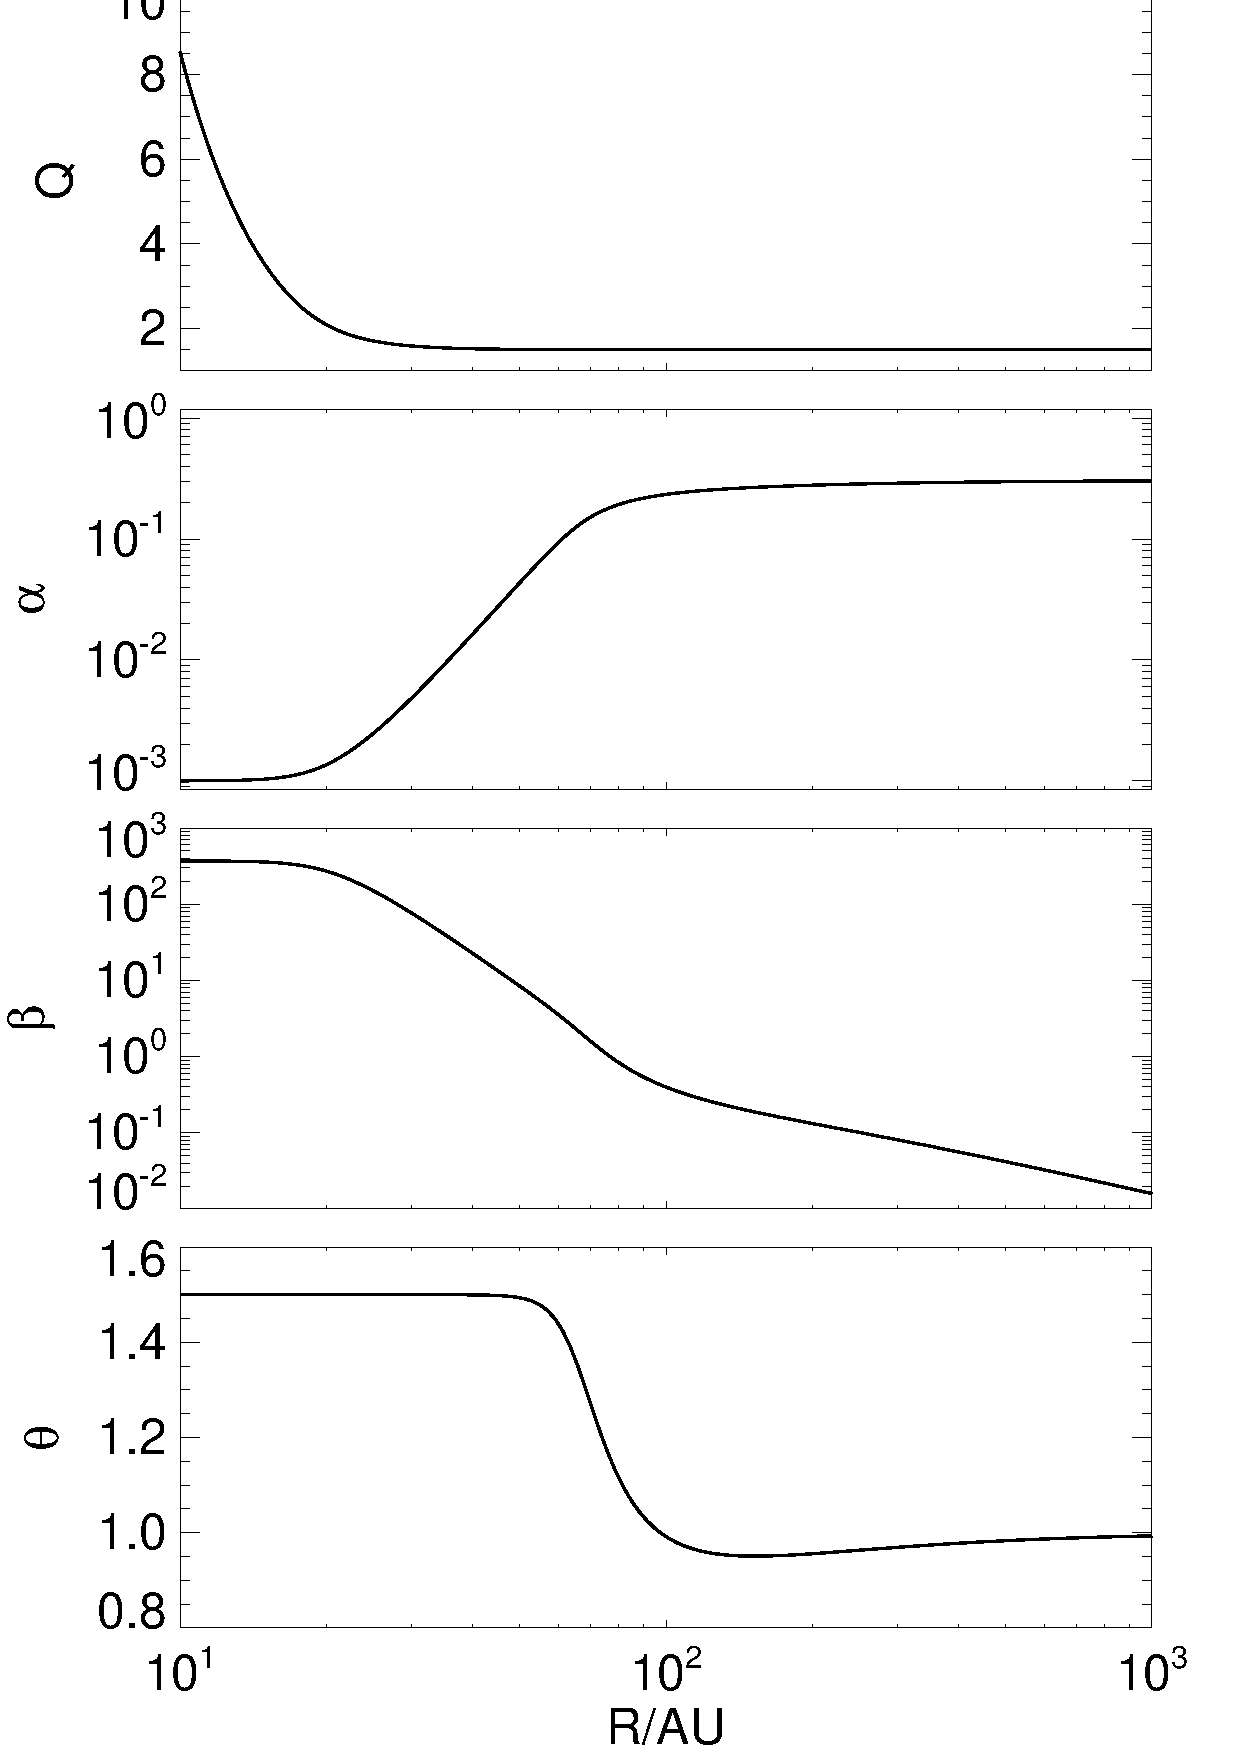
\includegraphics[width=\linewidth,clip=true,trim=0cm 0cm 0cm
    0.0cm]{figures/ppd_2d_basic}
  \caption{Equilibrium profile obtained from the disk model developed
    by \cite{rafikov15}, with parameters $\dot{M} =
    10^{-6}M_\sun\yr^{-1}$, $Q_0=1.5$, $\tirr=10\mathrm{K}$, and
    $\alpha_m=10^{-3}$.   
    \label{rafikov_model}}
\end{figure}

\begin{figure}
  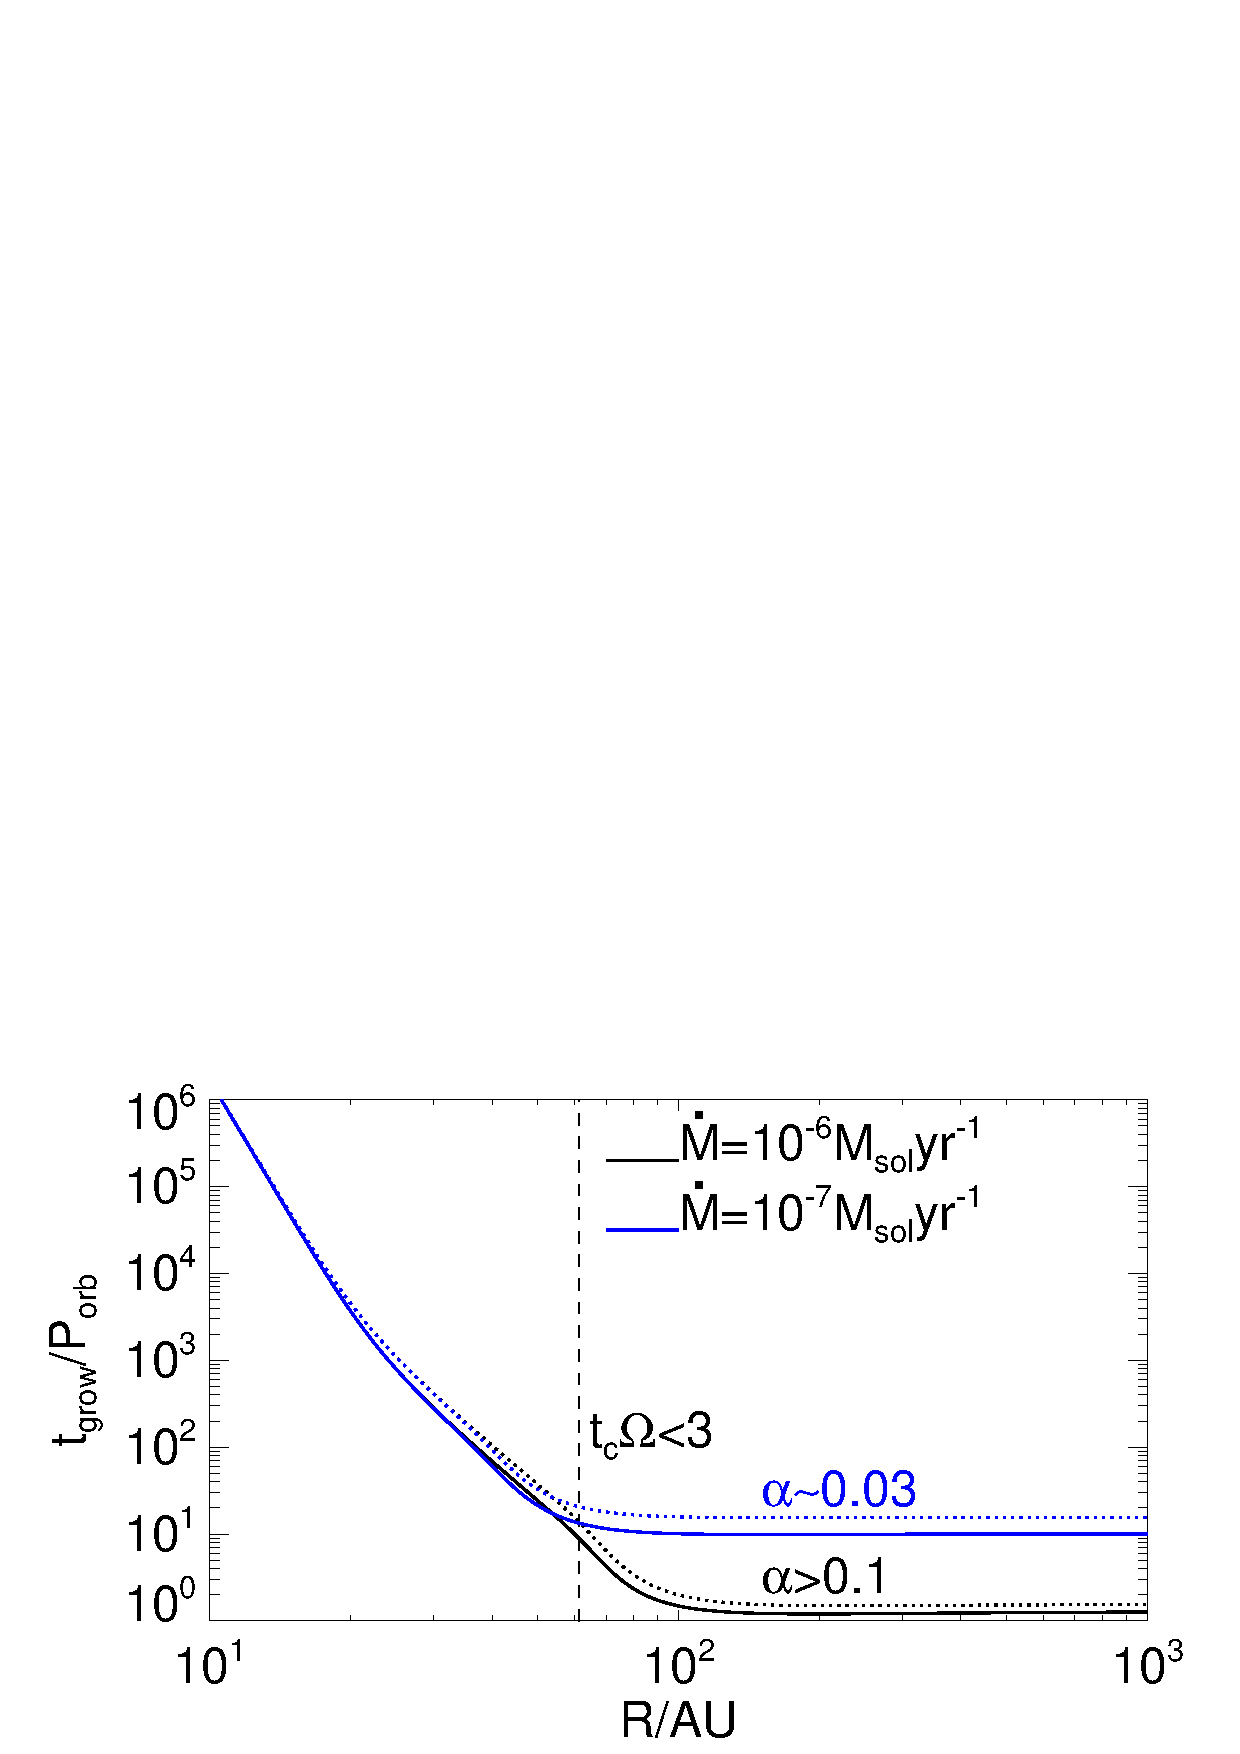
\includegraphics[width=\linewidth,clip=true,trim=0cm 1.5cm 0cm
    0.0cm]{figures/ppd_2d_growth}\\
  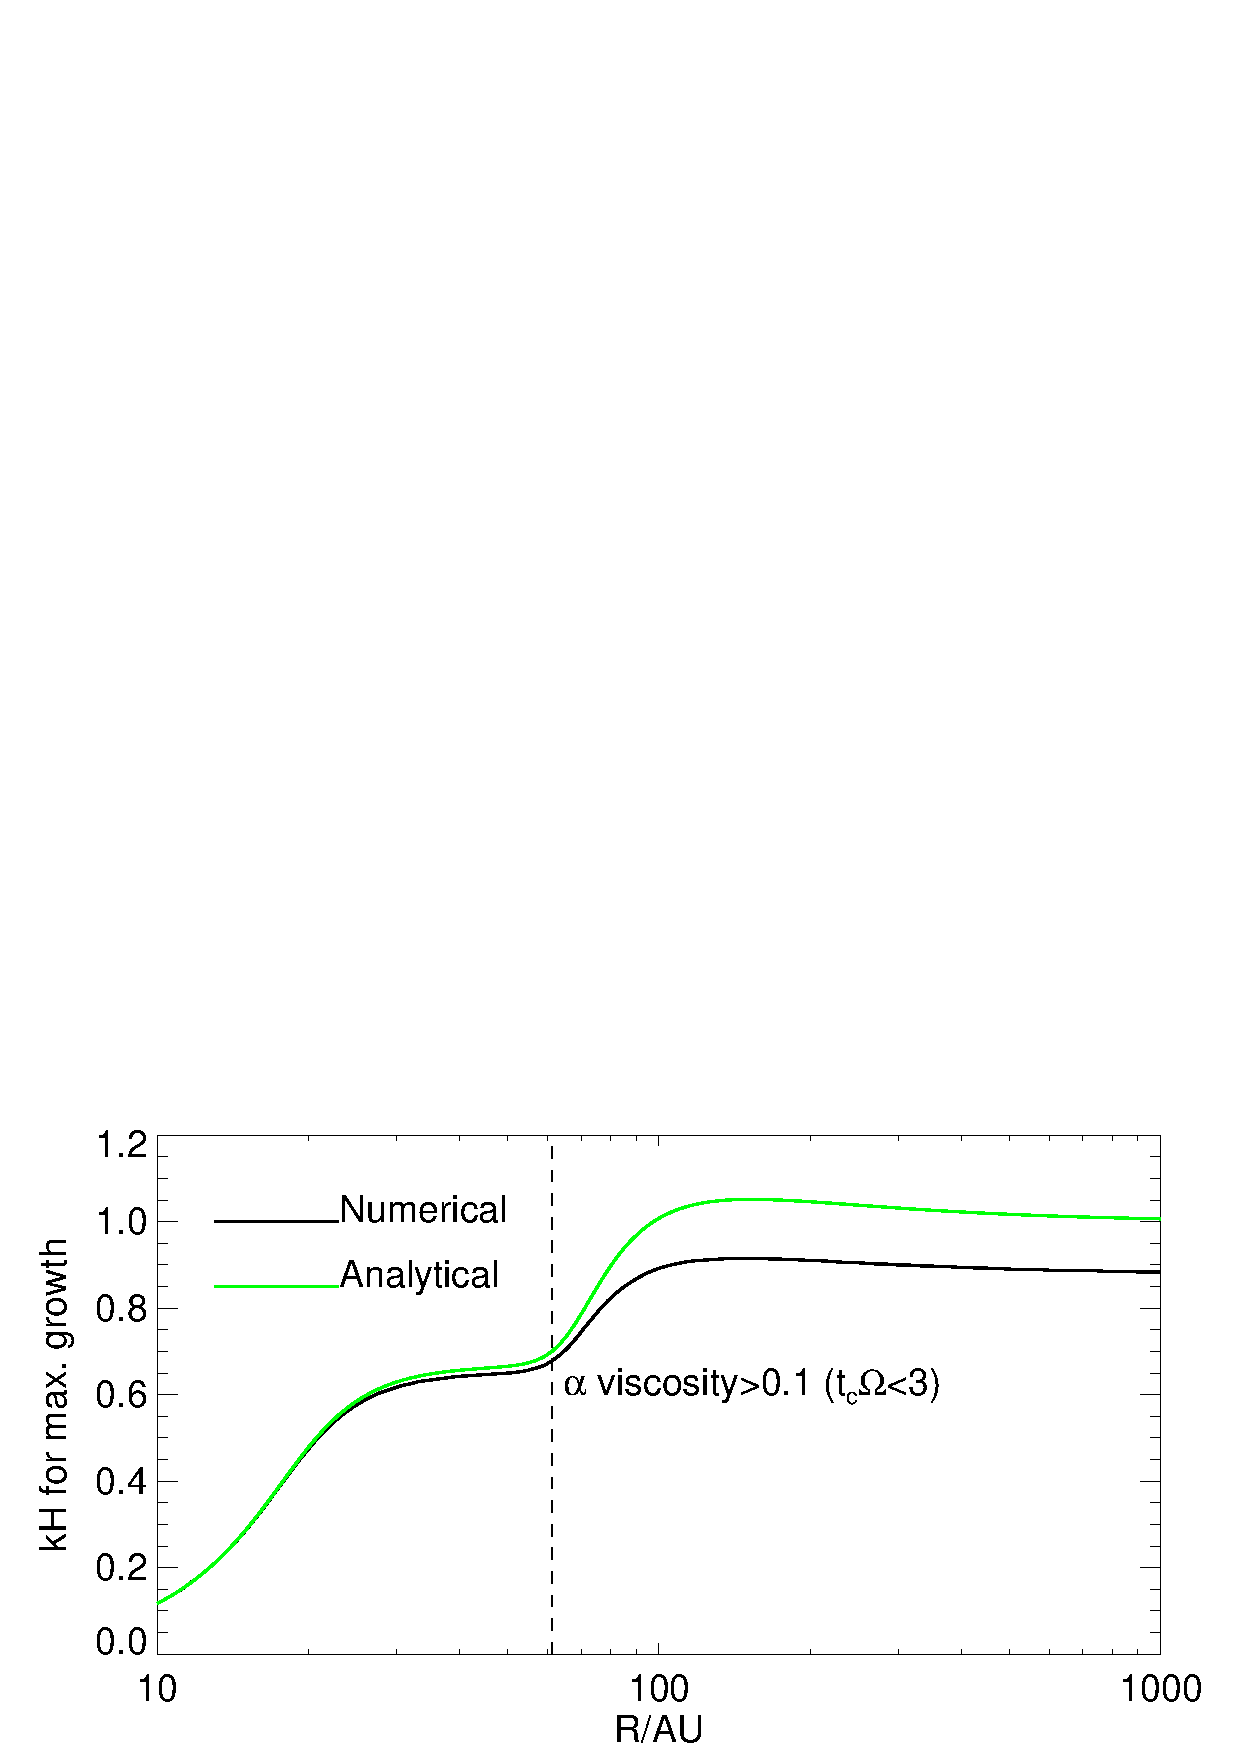
\includegraphics[width=\linewidth,clip=true,trim=0cm 0cm 0cm
    0.8cm]{figures/ppd_2d_maxk}
  \caption{Growth timescales (top) of the most unstable
    wavenumber (bottom) for viscous,
    self-gravitational modes in the 2D PPD model shown in
    Fig. \ref{rafikov_model}. 
    The black curve is obtained numerically
    from the 2D dispersion Eq. \ref{thindisk}, while green curves 
    are analytic results based on Eq. \ref{gammie_smallk}. 
    \label{rafikov_growth}}
\end{figure}


\subsection{3D PPD with radiative diffusion}
%appropriate for not-so-large distances where irrad can be neglected 
We briefly consider 3D PPDs with explicit radiative diffusion
(\S\ref{rad_cool}). 
Given the $\alpha(R)$ and $Q(R)$ profiles obtained
from the 2D model above, at each radius $R$ we obtain the vertical
structure from Eq. \ref{vert_eq1}---\ref{thermal_eq}, with 
Eq. \ref{rad_cool1}---\ref{rad_cool2} for the radiative flux.
We then solve the 3D eigenvalue problem as in \S\ref{3ddisk}, with the
additional boundary condition $\delta T^\prime(0) = \delta T(\zmax) = 0$.    
We use the same disk model as in \S\ref{pp2d_example} but 
with $T_\mathrm{irr}=0$, since our simple radiative diffusion model
does not include irradiation (\S\ref{rad_cool}). 
%physically, irrad is negligible for opt thick regions, and we are
%restricted to such regions if applying rad diff
We use a slightly smaller vertical
domain with $\rho(\zmax)=0.1\rho_0$.  %to avoid very low density 

Fig. \ref{rafikov_growth3d} show the growth rates and most unstable
wavenumber for $R\in[10,100]$AU; along with corresponding 2D 
results with softened self-gravity. There is a close match for
$R\lesssim60$AU where the disk is optically thick ($\tau\gtrsim
1$) and both models apply. However, beyond $60$AU where the disk
becomes optically-thin, radiative diffusion (the 3D curve) is not
valid and under-estimates the growth rates. %; while the $f(\tau)$
%function approximately captures opticall-thin cooling in the 2D case.  
However, the comparison shows that the transition radius
$R_t\sim60$AU can be correctly calculated within the 2D framework.  
%notice the small softenings used 
%This is not surprising since the
%instability is fundamentally driven by viscous and self-gravity forces in the
%momentum equations, not the energy equation. 

\begin{figure}
  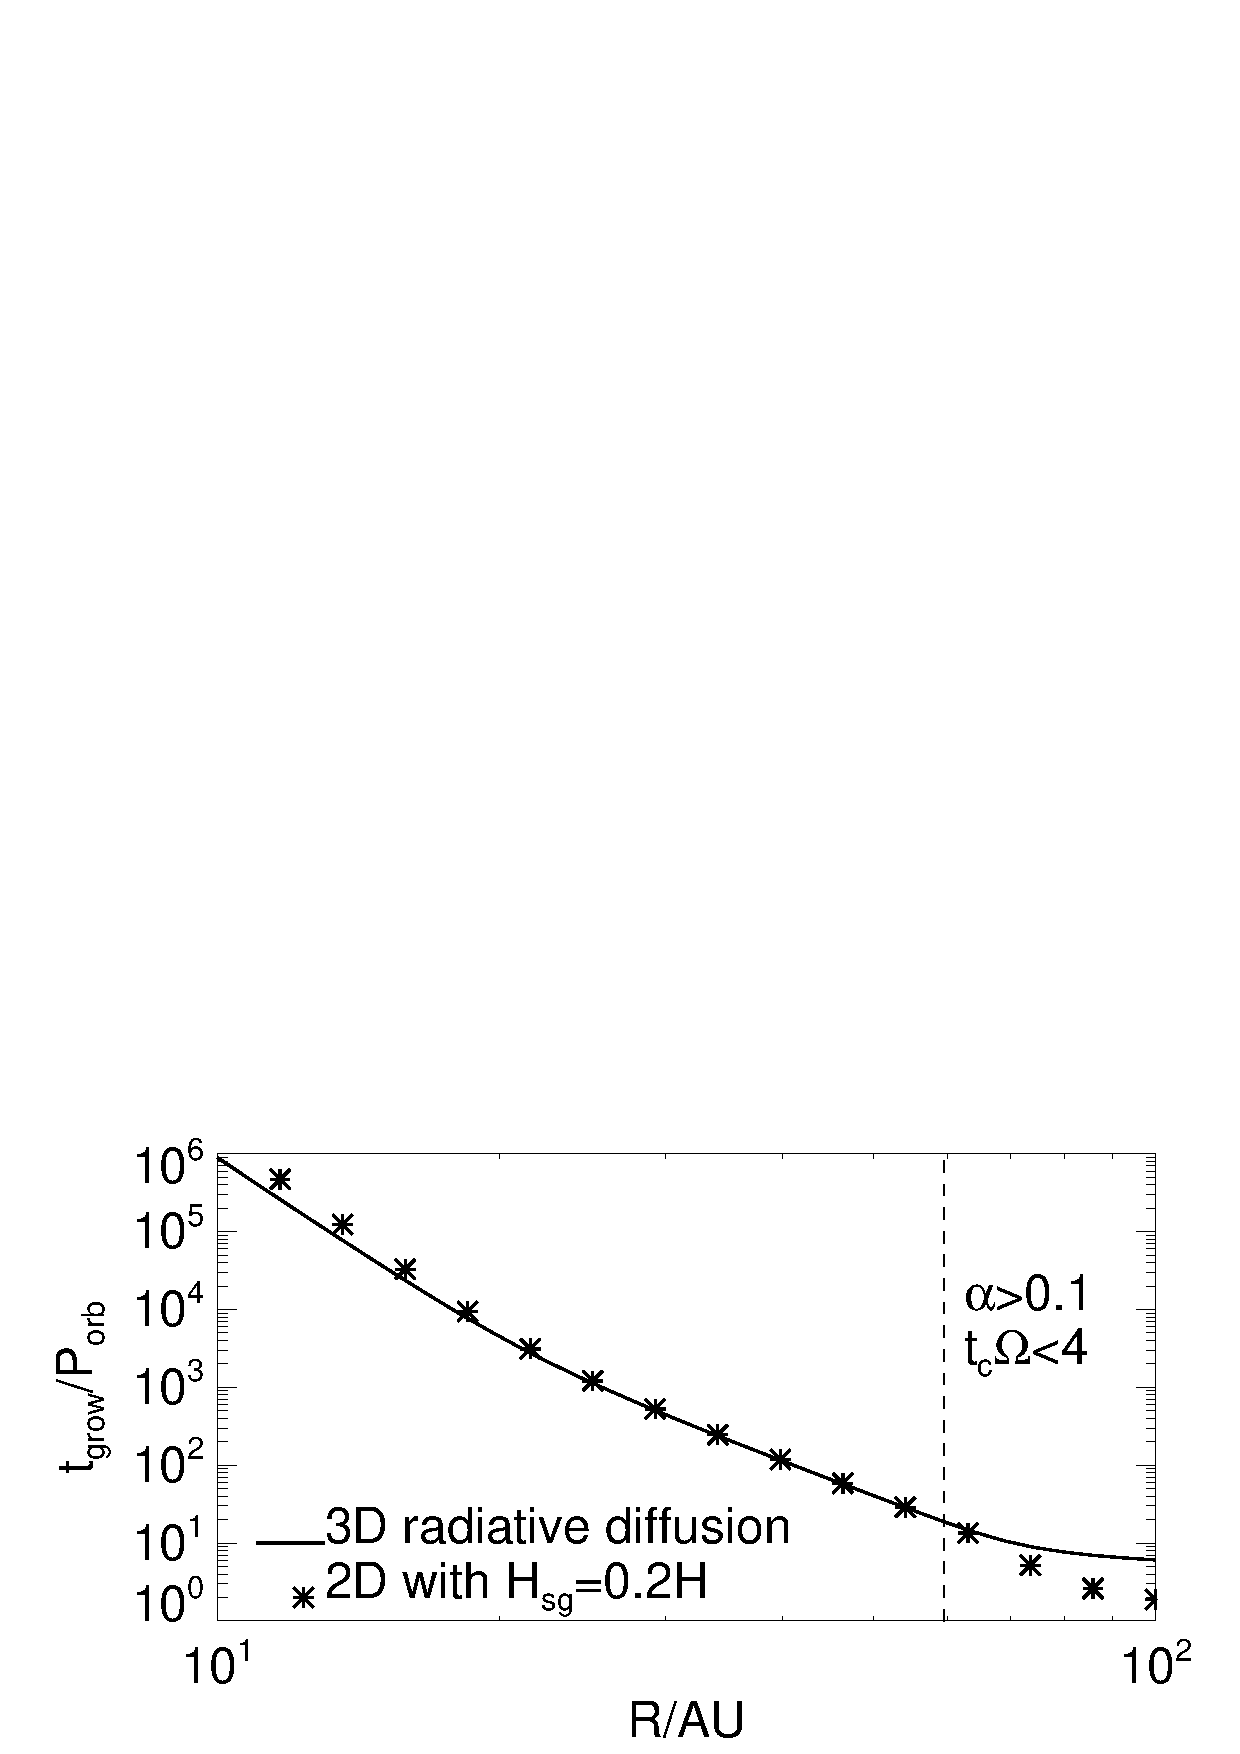
\includegraphics[width=\linewidth,clip=true,trim=0cm 1.5cm 0cm
    0.0cm]{figures/ppd_3d_rates}\\
  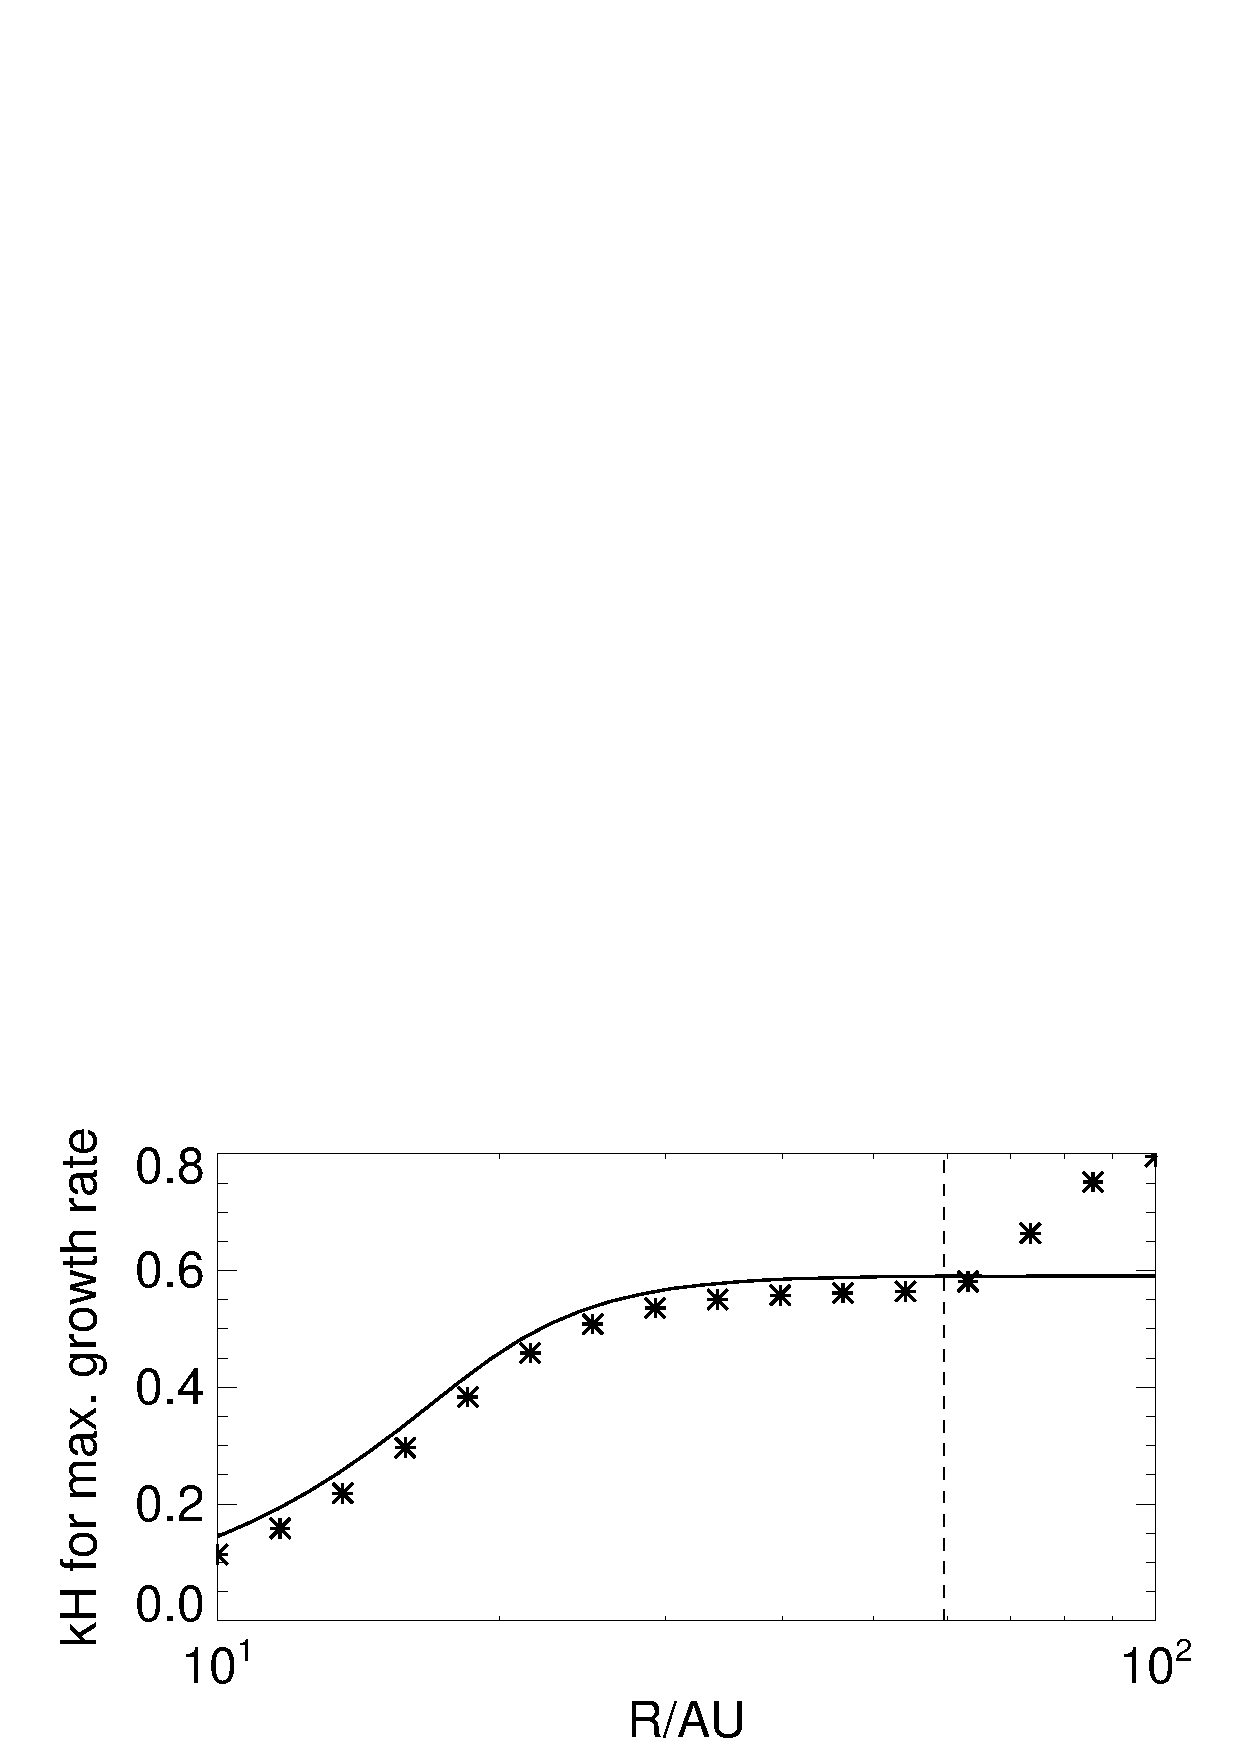
\includegraphics[width=\linewidth,clip=true,trim=0cm 0cm 0cm
    0.8cm]{figures/ppd_3d_maxk}
  \caption{Growth timescales (top) of the most unstable
    wavenumber (bottom) for viscous, 
    self-gravitating modes. The black curves are obtained
    from the 3D eigenvalue problem with radiative diffusion,
    applicable to optically-thick regions ($R\lesssim 60$AU); 
    while the green curves are obtained from the 2D corresponding
    model, which is applicable to both optically-thick and
    optically-thin regimes.  
    \label{rafikov_growth3d}}
\end{figure}



 
\section{Summary and discussion}\label{summary}
In this paper, we study the implications on the stability of
turbulent, cooling accretion disks if said turbulence is modeled as an
effective, Navier-Stokes viscosity. This viscosity provides a 
background heating and may also be active in the perturbed 
state. We pay particular attention to 
protoplanetary disks subject to `gravito-turbulence'. 
Our framework provide an alternative interpretation of existing
results on PPD fragmentation established from direct numerical
simulations. 
{\bf cooling removes pressure support, viscosity removes rotational support}
{\bf our conclusions do require input of emperical resuls from numerical
sims}

%generalized dispersion relation (inviscid)
%no magic beta - connection with stochastic 

We derive the disperion relation for local axisymmetric density waves 
subject to external heating and cooling (Eq. \ref{inviscid}), but
without viscous effects on the waves. We find
the sufficient condition for stability 
is \emph{independent} of the cooling rate. Long cooling times can
formally lead to instability, but the growth timescales may be
uninterestingly long. We obtain an analytic expression for the
dimensionless cooling time, $\beta_*$, required to remove pressure
support against self-gravity on radial lengthscales comparable to the 
disk scale height. We find $\beta_*$ reproduces the fragmentation
boundary found in previous numerical simulations (Table
\ref{bstar_compare}).  

%viscous GI ad connection with frag

We then include viscosity in the linear problem and generalize the
`viscous gravitational instability', previously discussed in 
simpler disk models \citep{lynden-bell74,gammie96,hunter83}, to include
heating/cooling and three-dimensionality. Our generalized framework is
readily applied to realistic protoplanetary disk models. For
gravito-turbulent PPDs, we find viscous GI grows on orbital time-scales
beyond $\sim 100\mathrm{AU}$. This means the assumed gravito-turbulent
steady state should not exist beyond dynamical time-scales in the
outer parts of PPDs. 

%viscosity > 0.1, beta < 3 - 4 

Our results bear striking similarities with the current consensus on
PPD fragmentation. It is generally accepted that PPDs can fragment
beyond a few tens of $\mathrm{AU}$. This conclusion results from
applying a Toomre stability condition (e.g. $Q\lesssim 1.5$) and a
cooling time or viscosity criteria (e.g. $\beta\lesssim 3$ or
$\alpha\gtrsim 0.1$), the latter of which is
based on numerical simulations. We find these
emperical conditions essentially translates to viscous GI on dynamical
time-scales. This suggests that gravito-turbulent
PPDs fragment because the associated viscous stresses further
destabilize the disk against self-gravity. 


%ultimately: why do disks fragment? viscosity may play a role

\subsection{Relation to numerical simulations}\label{prev_works}

\subsection{Other sources of turbulence}
%application to gravito-turbulence but actually linear theory does not assume
%actually application to 
%MHD turbulence prob makes more sense 
%require `scale separation' for GI turbulence (small-scale GI provide
%turbulence, large-scale GI for fragmentation)

\subsection{Outstanding issues}
%non-axisymmtric problem 
%viscosity model (maybe it doesn't behave like a power law)
%chosen a particular mu and lambda 



%\acknowlegement
%S. Stahler 

\appendix
\section{2D dispersion relation}\label{2ddisp}
The functions in Eq. \ref{thindisk} are 
\begin{align}
  A(S,K) =& \left(\frac{4}{3}\alpha+\alpha_b\right) K^2 + S +
  \mathcal{E}\mathcal{F}\label{bigA}
  - \frac{2|K|}{QS}, \\
  B(S,K) =& 2\left(\alpha q \mathcal{F} - 1\right),\\
  C(S,K) =& (2 - q) + \frac{\alpha q K^2(1+\mu)}{S} 
  + \alpha q \lambda \mathcal{E}\mathcal{F},\\
  D(S,K) = & \alpha K^2 + S + 2\alpha^2q^2\lambda\mathcal{F},
\end{align}
with
\begin{align}
  \mathcal{E} = \frac{\alpha q^2(1+\mu)}{S} +
    \frac{\gamma}{\gamma-1} + \frac{\theta}{\beta S(\gamma-1)},\quad
  \mathcal{F} = \frac{K^2(\gamma-1)\beta}{1 + \beta S - \alpha\beta
    q^2\lambda(\gamma-1)}\label{bigF}. 
\end{align}

\section{2D viscous GI} \label{gammie_check}
We obtain the dispersion relation for viscous GI described by
previous authors \citep{lynden-bell74,willerding92,gammie96} as 
follows. We set $\mu=-1, \lambda=0$ to obtain the same viscosity
models. Next we consider $|\beta S|\to \infty$, i.e. no explicit
cooling on the perturbations. Then the condition $AD = BC$ imply 
\begin{align}
  S^3 + \left(\frac{7}{3}\alpha + \alpha_b\right)K^2S^2 + \left[2(2-q) -
    \frac{2|K|}{Q} + \gamma K^2 + \alpha K^4 \left(\frac{4}{3}\alpha +
    \alpha_b\right)\right]S + \alpha K^2 \left[\gamma K^2 -
    \frac{2|K|}{Q} - 2q(2-q)(\gamma-1)\right]=0,
\end{align}
which agrees with \citet[Eq. 11]{willerding92} in the isothermal
limit ($\gamma=1$). The non-isothermal term $\propto (\gamma-1)$
originates from viscous dissipation which was excluded in the
aforementioned works. Its effect is to increase the maximum wavenumber 
for viscous GI. %it acts to stabilize 

An approximate solution for the growth rate may be obtained for small
$|K|$ by balancing the last two terms,
\begin{align}
  S \simeq \frac{\alpha K^2\left[2|K|/Q- \gamma K^2 + 
     2q(2-q)(\gamma-1)\right]}{2(2-q)  - 2|K|/Q + \gamma K^2 }, 
\end{align}
which coincides with \citeauthor{gammie96}'s Eq. 18 for $\gamma=1$. 

%In
%that case the condition for instability is
%\begin{align}
%%  \frac{2|K|}{Q} - K^2>0. 
%  |K|< \frac{2}{Q}.
%\end{align} 
%This is the same stability condition as if rotation was neglected in
%the standard, isothermal dispersion relation for density waves
%(obtained from Eq. \ref{thindisk} by setting $\gamma=\theta=1$). Thus
%the effect of viscosity is to remove 
%rotational stabilization against self-gravity, as originally explained
%by \cite{lynden-bell74}.  

%We recover \cite{gammie96}'s dispersion relation 
%for viscous gravitational instability as follows.  Next we
%simplify Eq. \ref{bigA}---\ref{bigF} by assuming $|\beta S |\gg 1$  
%This will turn out to be equivalent to $\beta\gg 1$, i.e. the
%adiabatic limit. 
%and $S\lesssim O(K^2)$ as $|K|\to 0$. Applying these considerations to
%Eq. \ref{thindisk} gives 
%\begin{align}
%  S = \frac{\alpha K^2\left[\frac{2|K|}{Q} - \gamma K^2 +
%      2q(2-q)(\gamma-1)\right]}{2(2-q) + \gamma K^2 - \frac{2K}{Q}}, 
%\end{align}
%which does not explicitly depend on cooling. 
%Setting $\gamma=1$ then gives \citeauthor{gammie96}'s Eq. 18. The above
%is expression thus generalizes \citeauthor{gammie96}'s result to
%non-isothermal disks. 

%cooling is not the physical cause of instability 

\section{3D corrections in 2D theory}\label{3dcorr}
The simplest way to mimic the effect of finite disk thickness
on gravitational instabilities is to weaken self-gravity by reducing 
the gravitational constant  
\begin{align}
  G \to G\left(1+|k|H_\mathrm{sg}\right)^{-1}, 
\end{align}
or equivalently $Q\to Q\left(1+|k|H_\mathrm{sg}\right)$. This
prescription, derived by \cite{shu84}, is widely applied
\citep[e.g.][]{youdin11,takahashi14}. Here $H_\mathrm{sg}$ is a
measure of the disk thickness. We intuitively expect
$H_\mathrm{sg}\sim H$, but its precise value is not known a priori.   
We regard $H_\mathrm{sg}$ as a free parameter of the problem.    


\section{Numerical method for the 3D eigenvalue problem}
We use a pseudo-spectral method to solve the set of ordinary
differential equations, Eq. \ref{lin_mass}---\ref{lin_gravity}, on 
the domain $ z\in[0,\zmax]$ with a parity condition at the midplane.
We expand $\bm{U}=[\delta P,\delta\rho,\delta\Phi,
  \delta v_x, \delta 
  v_y]$ in even Chebyshev polynomials,
\begin{align}
  \bm{U}(z) = \sum_{j=1}^N \bm{a}_jT_{2(j-1)}(z/\zmax), 
\end{align}
and the vertical velocity in odd Chebyshev polynomials,
\begin{align}
  \delta v_z(z) = \sum_{j=1}^N b_jT_{2j-1}(z/\zmax),   
\end{align}
where $\bm{a}_j$ and $b_j$ are the spectral coefficients. 
The basis functions are chosen to satisfy a reflecting boundary
condition at the midplane, %GI has even symmetry across midplane 
\begin{align}
  \bm{U}^\prime(0) = \bm{0}, \quad \delta v_z(0) = 0.
\end{align}
%At the upper disk boundary we also apply reflection,
We explicitly apply a reflecting upper disk boundary, 
\begin{align}
  \delta v_z(\zmax) = \delta v_x^\prime(\zmax) = \delta
  v_y^\prime(\zmax) = 0,
\end{align}
and the potential satisfies
\begin{align}
  \delta \Phi^\prime (\zmax) + k \delta\Phi(\zmax) = 0, 
\end{align}
as derived by \cite{goldreich65a} and used in similar studies  
\citep{kim12,lin14c}. %reflection is standard in direct simulations 

We discretize the equations, including upper disk boundary conditions,
over the $N$ positive abscissae of the extrema of $T_{2N-1}$. This
procedure converts the differential equations into a generalized
eigenvalue problem, for which we use the standard matrix package
LAPACK to solve. We use $N=65$. 


\bibliographystyle{apj}
\bibliography{ref}


\end{document}

